\documentclass[preprint,authoryear,11pt]{elsarticle}

\usepackage[charter]{mathdesign}
\let\circledS\undefined

% Page layout: same as the reference template
\usepackage[
  left=2.5cm,
  right=2.5cm,
  top=3cm,
  bottom=2.8cm
]{geometry}

\usepackage{amsmath,amsthm,bm}
\usepackage{soul}
\usepackage{graphicx}
\usepackage{rotating}
\usepackage{indentfirst}
\usepackage{setspace}
\usepackage{footmisc}
\usepackage{paralist}
\usepackage{multirow,multicol}
\usepackage{booktabs,threeparttable}
\usepackage{caption,subcaption}
\usepackage{bbding}
\usepackage[section]{placeins}
\usepackage{array,tabularx}
\usepackage{natbib}
\usepackage{afterpage}
\usepackage{appendix}
\usepackage{tikz}
\usetikzlibrary{patterns,calc}
\usepackage[section]{algorithm}
\usepackage{algorithmic}
\usepackage{cases}
\usepackage[mathcal]{eucal}
\usepackage{lscape,pdflscape}
\usepackage{makecell}
% Packages used in the TRC manuscript
\usepackage{float,adjustbox}
\usepackage{dsfont,physics}
\usepackage[table]{xcolor}
\usepackage{hyperref}
\usepackage{longtable}
\pdfstringdefDisableCommands{%
  \def\corref#1{}%
  \def\citep#1{}%
}

\setlength{\footnotesep}{\baselineskip}
\renewcommand{\footnotelayout}{\doublespacing}
\allowdisplaybreaks[4]

\setlength{\parindent}{2em}
\setlength{\parskip}{0.5em}
\onehalfspacing

\newtheorem{theorem}{Theorem}
\newtheorem{theorem2}{Theorem2}
\newtheorem{prop}{Proposition}
\theoremstyle{definition}
\newtheorem{definition}{Definition}
\newtheorem{lemma}[theorem]{Lemma}
\newtheorem{remark}[theorem2]{Remark}
\newtheorem{conjecture}[theorem2]{Conjecture}
\newtheorem{corollary}{Corollary}
\newtheorem{example}{Example}

\newcounter{subsubsubsection}[subsubsection]
\renewcommand{\thesubsubsubsection}{\alph{subsubsubsection}}
\newcommand{\subsubsubsection}[1]{%
  \refstepcounter{subsubsubsection}%
  \textit{\thesubsubsubsection)} #1%
}

\definecolor{rred}{RGB}{204,0,0}
\definecolor{ggreen}{RGB}{0,145,0}
\definecolor{yyellow}{RGB}{255,185,0}
\definecolor{bblue}{rgb}{0.2,0.2,0.7}
\definecolor{bestgray}{gray}{0.88}
\newcommand{\best}[1]{\cellcolor{bestgray}#1}
\newcommand{\second}[1]{\underline{#1}}

% As in the reference template, line numbers are off.
% \usepackage{lineno}

\journal{Transportation Research Part C: Emerging Technologies}
\date{}

\begin{document}
\begin{frontmatter}

\title{An Explainable Framework for Points of Interest (POI) Demand Forecasting with Temporal Graph Networks}

\author[a]{Xu Liu}
\ead{xuliu8@uw.edu}

\author[b]{Yida Xu\corref{cor1}}
\ead{yida0101@uw.edu}

\author[c]{Cynthia Chen}
\ead{qzchen@uw.edu}

\cortext[cor1]{Corresponding author. Email address: yida0101@uw.edu (Yida Xu)}

\address[a]{Department of Statistics, University of Washington,
Seattle, WA 98195, USA}
\address[b]{Department of Industrial and Systems Engineering,
University of Washington, Seattle, WA 98195, USA}
\address[c]{Department of Civil and Environmental Engineering,
University of Washington, Seattle, WA 98195, USA}


\begin{abstract}
Points of interest (POIs), such as stores, clinics, and transit facilities, show where people access urban services and engage in daily activities.
Their visit counts describe how activity varies across locations and time, providing information for local mobility and service planning.
In practice, many POIs have sparse or intermittent visit histories, making future activity difficult to forecast from their own past observations.
Even when statistical or machine learning models forecast POI visits accurately, explaining their predictions and identifying the underlying information sources remain challenging.
To address these challenges, we develop an explainable temporal graph framework to forecast POI visits and examine when information from related POIs improves predictions and how model behavior varies across locations.
Using 92 days of data for 9,884 POIs in Seattle, we apply Evolving Graph Convolutional Networks (EvolveGCN) and Multivariate Time Series Graph Neural Networks (MTGNN) to forecast POI visits while incorporating spatial, functional, and visit-based relationships among POIs.
The forecasting results show that MTGNN achieves the lowest mean absolute error (MAE) across four input-window and forecast-horizon settings, while EvolveGCN with identity adjacency achieves greater positive-demand recovery among low-history POIs at the cost of more false activations.
Neighbor-group perturbations further reveal that recently active neighbors contribute to both positive-demand recovery and false activation.
We use gradient-based feature attribution to characterize how historical visits and static attributes contribute to individual predictions, revealing heterogeneous attribution patterns across POIs and urban functions.
Finally, we examine parent-place information and compare category labels and industry codes at different levels of granularity.
The results show that parent-place information provides a supplementary predictive signal, while broad industry classifications dominate semantic attribution and more specific functional connections are associated with fewer spurious transfers.
\end{abstract}


\end{frontmatter}

\section{Introduction}\label{intro}

Points of interest (POIs), such as stores, clinics, and transit facilities, show where people access urban services and engage in daily activities. 
Their visit counts describe how activity varies across locations and time, providing potential information for local mobility and service planning. 
To anticipate changes in demand and support transportation and local service planning, one can forecast future POI visits by leveraging historical visit counts \citep{hajisafi2023learning}.
However, sparse or intermittent visit histories (e.g., frequent zero-visit days with only occasional positive counts) make future activity difficult to forecast from a POI's own past observations \citep{turkmen2021forecasting,zhuang2022uncertainty}. Some studies therefore use information from related POIs to improve forecasts \citep{hajisafi2023learning}, but connecting a POI to distant locations may cause over-smoothing (e.g., producing near-identical forecasts for POIs with different visit patterns), and directly using neighboring visit counts may lead to over-prediction (e.g., forecasting substantially more visits than the POI actually receives) for POIs with limited histories \citep{zhang2026causalpoi}.

To address these challenges, machine learning (ML) models have been introduced to learn shared patterns across POIs while using each POI's visit history and attributes to distinguish its own activity.
These models represent visit observations and POI attributes as feature vectors and learn how these inputs relate to future visit counts.
Notably, recurrent models process historical inputs sequentially by updating hidden states that summarize earlier observations, allowing recent and earlier visits to inform forecasts \citep{hochreiter1997long}. 
Graph neural networks (GNNs) further represent each POI as a \textit{node} with its own feature vector and relationships among POIs as \textit{edges}. 
The edge weights form an \textit{adjacency matrix}, which specifies which POIs exchange information and the relative strength of their connections \citep{hajisafi2023learning}.
Selecting and weighting these connections based on spatial proximity and functional similarity can limit noisy relationships among POIs and reduce over-smoothing.
For POIs with sparse or intermittent visit histories, scaling adjacency weights derived from neighboring POIs can also reduce over-prediction \citep{zhang2026causalpoi}.

POI visits exhibit both spatial and temporal dependencies across locations and over time.
To capture spatial and temporal dependencies jointly, some studies have begun using spatiotemporal graph neural networks (ST-GNNs) for POI visit forecasting \citep{hajisafi2023learning,zhang2026causalpoi}.
Representative architectures include Evolving Graph Convolutional Networks (EvolveGCN) and the Multivariate Time Series Graph Neural Network (MTGNN). 
EvolveGCN recurrently updates graph-convolution parameters across input days \citep{pareja2020evolvegcn}, while MTGNN learns relationships among time series and uses temporal convolutions to capture lagged patterns \citep{wu2020connecting}. 
These models provide a natural framework for POI visit forecasting by jointly modeling visit histories and relationships among POIs.
We therefore use EvolveGCN and MTGNN to predict future visit counts for individual POIs.

For urban planners and transportation agencies, forecasting future POI visits provides information about expected demand, while understanding what drives those forecasts can offer additional guidance for service planning and operational decisions \citep{hajisafi2023learning}. 
For example, visits to a clinic may be driven more by its functional identity than by its location, so opening a restaurant at the same site may not necessarily attract the same level of customer traffic. 
Meanwhile, the parent-place context of a clinic within a larger medical facility may also contribute to its predicted visits.
Therefore, understanding what drives predicted visits can help decision makers assess whether demand is tied to the location itself or to the specific type of POI operating there.
Yet neural forecasting models are often treated as black boxes because their prediction processes are difficult to interpret \citep{ribeiro2016should,lipton2018mythos}. In particular, it is hard to tell whether a high forecast for a sparse POI reflects useful evidence of future visits or excessive reliance on activity at related locations.

In recent years, developments in explainable artificial intelligence (XAI) provide tools for examining the information behind individual predictions. One widely used approach is \textit{feature attribution}, which estimates the contributions of input features to a model output and has been applied to image and text models to help users uncover latent information underlying their predictions \citep{ribeiro2016should,pmlr-v70-sundararajan17a}. 
Among feature attribution methods, gradient-based approaches are particularly suitable for high-dimensional differentiable models, as they can evaluate many input features through backpropagation without repeatedly modifying inputs and rerunning the model as required by perturbation-based methods \citep{pmlr-v70-sundararajan17a,ivanovs2021perturbation}.  
This computational efficiency also enables fine-grained analysis across historical days and POI attributes. Specifically, gradient-based approaches backpropagate from a target prediction to the input and use the resulting gradients to quantify how sensitive that prediction is to individual input features. 
We therefore use gradient-based attribution to identify which inputs drive POI visit predictions, assign POIs to attribution regimes according to their relative feature contributions, and examine how these contributions vary across POI types and urban contexts.

Using a dataset that includes 92 days of observations for 9,884 POIs in Seattle, we develop an explainable forecasting framework that combines EvolveGCN and MTGNN with gradient-based feature attribution. 
To examine how different relationships among POIs affect forecasting, we construct alternative adjacency matrices based on spatial proximity, functional similarity, and historical visit patterns, and perturb selected neighbor groups to assess how their information changes individual forecasts. 
We next incorporate diverse POI-level attributes to investigate which characteristics drive individual predictions.
To further examine forecasting behavior when historical information is sparse, we focus particularly on \textit{low-history POIs}, identified by frequent zero visits and small positive historical averages during training. 
Based on these preliminary analyses, this study aims to address four research questions:
\begin{compactenum}
    \item \textbf{How do temporal graph models perform relative to simpler forecasting methods across different historical input windows and forecast horizons, particularly for POIs with sparse visit histories?}
    \item \textbf{When does information from related POIs improve forecasts for low-history POIs, and when does it lead to over-prediction?}
    \item \textbf{Which information sources drive POI visit predictions, and how do these prediction mechanisms vary across POIs and urban functions?}
    \item \textbf{How do parent-place context and semantic information (i.e., category and industry classifications) at different levels of granularity contribute to POI visit predictions?}
\end{compactenum}

To answer the above questions, we conduct a sequence of forecasting and attribution experiments. 
We first compare EvolveGCN and MTGNN with historical-average, autoregressive ridge regression, and long short-term memory (LSTM) baselines across different historical input windows and forecast horizons \citep{hochreiter1997long}. 
In addition to aggregate forecasting error, we evaluate whether the models can recover positive visits for low-history POIs without over-predicting zero-visit observations, thereby examining \textit{zero-demand collapse}, defined as near-zero forecasts for observations with positive visits.
We then compare alternative graph structures and perturb selected groups of connected POIs to determine how information transferred from related POIs affects individual forecasts. 
Finally, we use gradient-based feature attribution to identify the information sources underlying POI predictions, assign POIs to attribution regimes, and examine the contributions of parent-place information and semantic attributes at different levels of granularity.


The results show that MTGNN achieves the lowest forecasting error across all four input-window and forecast-horizon settings, while EvolveGCN with identity adjacency recovers more positive demand mass among low-history POIs at the cost of more false activations.
For low-history POIs, information from related POIs can improve the recovery of positive visits, but such information can also raise predictions when no visits occur, indicating that graph-based transfer is not uniformly beneficial across prediction settings.
The attribution results reveal heterogeneous prediction mechanisms across POIs, with varying reliance on visit history, location, functional identity, parent-place context, and other static attributes.
Parent-place information generally provides supplementary predictive signals, while broad industry classifications show stronger semantic attribution and finer-grained functional connections are associated with fewer spurious transfers.


The remainder of the paper is organized as follows.
Section~\ref{lit} reviews the relevant literature.
Section~\ref{problem_setting} introduces the dataset and formulates the prediction and attribution tasks.
Section~\ref{sec:methodology} then describes the forecasting models and analytical methods.
Subsequently, Section~\ref{sec:results} presents the forecasting and attribution experiments.
Finally, Section~\ref{conclude} summarizes the findings and discusses future work.

\section{Literature Review}
\label{lit}

We review three streams of literature relevant to this study: POI visit forecasting, spatial and functional relationships among POIs, and explainable spatiotemporal forecasting.

\subsection{POI visit forecasting}
\label{lit_poi}
Existing studies on POI visit forecasting use historical visit records to predict future activity.
For example, \citet{hajisafi2023learning} compared historical-average and seasonal-naive forecasts with neural models for POI visit prediction.
Beyond such historical summaries, learning-based methods model temporal dependence directly from past observations.
\citet{salinas2020deepar} used an autoregressive recurrent model to represent sequential dependence, while \citet{zhang2017deep} incorporated recent observations, periodic patterns, and longer-term trends when forecasting urban crowd flows.
These studies show how forecasting models can move from simple historical summaries to richer representations of temporal dependence, allowing recent activity and recurring temporal structure to jointly inform future predictions.

Forecasting performance can also vary with the prediction horizon.
Longer-horizon forecasts are more likely to accumulate prediction errors \citep{sorjamaa2007methodology,taieb2014boosting}, motivating different multi-step forecasting strategies.
Recursive approaches repeatedly apply a one-step-ahead model, whereas direct approaches estimate separate predictions for different horizons \citep{marcellino2006comparison,chevillon2007direct}.
Because recursive forecasts may accumulate errors and direct forecasts require horizon-specific models, \citet{taieb2012review} examined multi-output and hybrid strategies that combine their advantages.
Multi-step traffic forecasting similarly shows that prediction performance can change as the forecast horizon increases \citep{wang2020forecast}.
We therefore evaluate POI forecasting performance across multiple forecast horizons.

A further challenge arises when POI visit histories are sparse or intermittent, with many zero-visit periods and only occasional positive observations.
To address such settings, \citet{croston1972forecasting} separated positive demand sizes from inter-arrival intervals, while \citet{syntetos2005accuracy} introduced a bias-adjusted estimator and \citet{teunter2011intermittent} updated demand-occurrence probabilities during zero-demand periods.
More recently, \citet{turkmen2021forecasting} combined renewal processes with recurrent neural networks, and \citet{zhuang2022uncertainty} modeled excess zeros in sparse origin--destination flows using a zero-inflated distribution.
Sparse observations also complicate evaluation: all-zero forecasts can perform well under some aggregate accuracy measures despite missing positive demand \citep{turkmen2021forecasting}.
For low-history POIs, aggregate error may therefore mask whether a model captures occasional positive visits or simply produces consistently small forecasts.

Motivated by these studies, we evaluate POI visit forecasts across different historical input windows and forecast horizons.
To examine whether models can recover positive visits without increasing false positive predictions, we compare temporal graph models with simpler baselines and separately evaluate positive- and zero-visit observations for low-history POIs.


\subsection{Spatial and functional relationships among POIs}
\label{lit_sfr}

In addition to a POI's own visit history, forecasting models can draw on information from related locations.
This raises the question of which locations should share information while preserving differences in their activity patterns.
To balance information pooling and unit-level heterogeneity, \citet{cohen2022data} developed a clustering approach that determines whether demand-model coefficients should be estimated at the individual, cluster, or aggregate level.
In spatial forecasting, \citet{yao2018deep} combined similarities in regional demand patterns with local spatial relationships, while \citet{geng2019spatiotemporal} used multiple graphs to represent different correlations among regions.
Some studies rely on predefined network structure \citep{li2018diffusion}, whereas others learn dependencies directly from data \citep{wu2019graph,bai2020adaptive}.

For POIs, relationships may arise from historical activity, geographic proximity, or functional characteristics. 
To identify useful connections while limiting irrelevant information, \citet{hajisafi2023learning} integrated geographic distance, historical visit patterns, textual attributes, and category relationships with mechanisms that filter noisy connections. 
\citet{zhang2026causalpoi} similarly used functional interactions with surrounding locations to supplement limited historical information for newly introduced POIs. 
However, excessive information sharing can make node representations increasingly similar and weaken location-specific visit patterns \citep{li2018deeper,oono2020graph}. 
This suggests that related-POI information is useful only when it supplements limited histories without obscuring meaningful differences in activity across locations.

POI context can also reflect whether an individual establishment is located within a larger containing place such as a shopping mall, airport, or stadium, i.e., parent-place relationships.
For example, \citet{gould2005contracts} examined customer externalities among tenants within shopping malls, suggesting that activity at an individual establishment may also be associated with its surrounding parent place.
Motivated by this relationship, we examine parent-place information as an additional source of context for POI visit forecasting.
We also compare category and industry classifications at different levels of detail to assess whether finer representations provide additional predictive information.


\subsection{Explainable spatiotemporal forecasting}
\label{lit_exp}

Recent XAI research has examined which inputs contribute to individual predictions.
One common approach is local explanation, which attributes model outputs to observed features.
Among these methods, \citet{ribeiro2016should} fitted interpretable surrogate models around individual predictions, while \citet{lundberg2017unified} developed an additive attribution framework based on Shapley values.
To further connect such explanations with operational decisions, \citet{senoner2022using} used attribution analysis to identify production processes associated with product quality and evaluated the resulting interventions through a field experiment.
These studies show how local explanations can reveal the information underlying individual model outputs.

For temporal and graph models, some studies have also examined how predictions depend on information across time, features, and connected units.
For example, \citet{bento2021timeshap} developed TimeSHAP to attribute recurrent predictions across features and time steps, while \citet{lim2021temporal} used variable selection and interpretable attention to examine temporal input relevance.
For graph predictions, \citet{ying2019gnnexplainer} identified influential subgraphs and node features, and \citet{luo2020parameterized} developed an explainer that can be applied across multiple graph instances.
To characterize broader model behavior, \citet{lundberg2020local} aggregated attribution profiles to identify groups with similar patterns of model reliance.
This approach provides a way to examine whether different observations systematically depend on different information sources.

To identify which information sources drive individual POI forecasts, we use gradient-based attribution to quantify the contributions of historical visits and static POI attributes.
We then assign POIs to attribution regimes according to their relative feature contributions to identify differences in the information sources underlying predictions.
To characterize these differences, we relate the resulting groups to POI characteristics and urban functions and examine how prediction mechanisms vary across locations.
Table~\ref{tab:literature_comparison} summarizes the research focus of representative studies across the three literature streams and highlights the scope of this study.

\begin{table}[!htbp]
\centering
\caption{Comparison of representative studies.}
\label{tab:literature_comparison}
\small
\renewcommand{\arraystretch}{1.08}
\begin{tabular*}{\textwidth}{@{\extracolsep{\fill}}lccccccc@{}}
\toprule
\textbf{Study} & \textbf{F} & \textbf{H} & \textbf{S} & \textbf{R} & \textbf{PC} & \textbf{E} & \textbf{G} \\
\midrule
\citet{gould2005contracts} &  &  &  & $\checkmark$ & $\checkmark$ &  & \\
\citet{taieb2012review} & $\checkmark$ & $\checkmark$ &  &  &  &  & \\
\citet{ying2019gnnexplainer} &  &  &  & $\checkmark$ &  & $\checkmark$ & \\
\citet{lundberg2020local} &  &  &  &  &  & $\checkmark$ & $\checkmark$ \\
\citet{bento2021timeshap} &  &  &  &  &  & $\checkmark$ & \\
\citet{lim2021temporal} & $\checkmark$ & $\checkmark$ &  &  &  & $\checkmark$ & \\
\citet{turkmen2021forecasting} & $\checkmark$ &  & $\checkmark$ &  &  &  & \\
\citet{zhuang2022uncertainty} & $\checkmark$ &  & $\checkmark$ & $\checkmark$ &  &  & \\
\citet{hajisafi2023learning} & $\checkmark$ &  &  & $\checkmark$ &  &  & \\
\citet{zhang2026causalpoi} & $\checkmark$ &  &  & $\checkmark$ &  & $\checkmark$ & \\
\midrule
\textbf{This study} & $\checkmark$ & $\checkmark$ & $\checkmark$ & $\checkmark$ & $\checkmark$ & $\checkmark$ & $\checkmark$ \\
\bottomrule
\end{tabular*}

\vspace{4pt}
\begin{minipage}{\textwidth}
\footnotesize
\textit{Notes:}
F: forecasting;
H: forecast-horizon comparison;
S: sparse or intermittent demand;
R: spatial, functional, or graph relationships;
PC: parent-place context;
E: local explanations of predictions or estimated effects;
G: grouping by attribution profiles.
\end{minipage}
\end{table}

\section{Data and Problem Formulation}
\label{problem_setting}

To answer the four research questions introduced in Section~\ref{intro}, we organize the empirical analysis into two complementary tasks. 
The \textit{prediction task} addresses the first research question by evaluating forecasting performance across historical input windows, forecast horizons, and POIs with different levels of historical activity. 
The \textit{attribution task} then addresses the remaining questions by examining when information from related POIs improves or worsens individual forecasts, which information sources drive POI predictions, and how parent-place context and semantic information at different levels of granularity contribute to these predictions. We first describe the dataset and then formulate the two tasks.


\subsection{Dataset and POI Attributes}
\label{subsec:data}

To capture both temporal visit patterns and heterogeneous POI characteristics, we use SafeGraph POI visit data from the Seattle metropolitan area.
The dataset contains daily observed visits from October to December 2020, covering \(92\) days and \(N=9{,}884\) POIs.
Each POI is represented by its daily visit counts together with a collection of static attributes describing geographic location, functional identity, organizational context, and operating conditions.

Geographic information is represented by latitude and longitude, which can be used directly as node features or to construct spatial relationships among POIs.
Functional identity is represented using SafeGraph top-level categories, sub-categories, and North American Industry Classification System (NAICS) codes.
We additionally use two-digit (NAICS-2) and four-digit (NAICS-4) NAICS prefixes to represent industry classifications at different levels of granularity.
For example, a supermarket with NAICS code 445110 is classified under NAICS-2 code 44 (Retail Trade) and NAICS-4 code 4451 (Grocery Stores).

Brand information identifies POIs associated with recognizable chains or branded establishments.
This information can capture common commercial identity even when two locations are geographically separated.
Parent-place information represents containment relationships between POIs.
For example, an individual store may be located inside a shopping mall, a restaurant inside an airport, or a clinic inside a larger medical facility.
Such relationships differ from ordinary functional similarity because the target POI is physically embedded within a larger destination.
Opening-hour information describes the regular operating schedule of each POI.
As opening-hour information is unavailable for some locations, we also retain a missingness indicator as a separate input.
Table~\ref{tab:poi_attributes} summarizes the POI attributes used in the analysis.

\begin{table}[ht]
\centering
\caption{Summary of POI attributes in the SafeGraph dataset.}
\label{tab:poi_attributes}
\small
\begin{tabular*}{\textwidth}{@{\extracolsep{\fill}}lll@{}}
\toprule
\textbf{Variable label} & \textbf{Interpretation} & \textbf{Example} \\
\midrule
$\mathrm{lat}_j, \mathrm{lon}_j$
& Geographic coordinates of POI \(j\)
& \((47.65,-122.31)\) \\

$\mathrm{cat}_j$
& Top-level POI category label
& Grocery Stores \\

$\mathrm{naics2}_j$
& Two-digit NAICS industry prefix
& 44 \\

$\mathrm{naics4}_j$
& Four-digit NAICS industry prefix
& 4451 \\

$\mathrm{naics}_j$
& Full six-digit NAICS code
& 445110 \\

$\mathrm{subcat}_j$
& Sub-category label from the full NAICS code
& Supermarkets and Other Grocery Stores \\

$\mathrm{brand}_j$
& Brand name associated with POI \(j\)
& Starbucks \\

$\mathrm{parent}_j$
& Larger containing place of POI \(j\)
& Mall, airport, or stadium \\

$\mathrm{open}_j$
& Regular opening-hour information
& Monday 8:00--18:00 \\
\bottomrule
\end{tabular*}
\end{table}

\begin{figure}[!htb]
\centering
\begin{subfigure}[t]{0.49\textwidth}
    \centering
    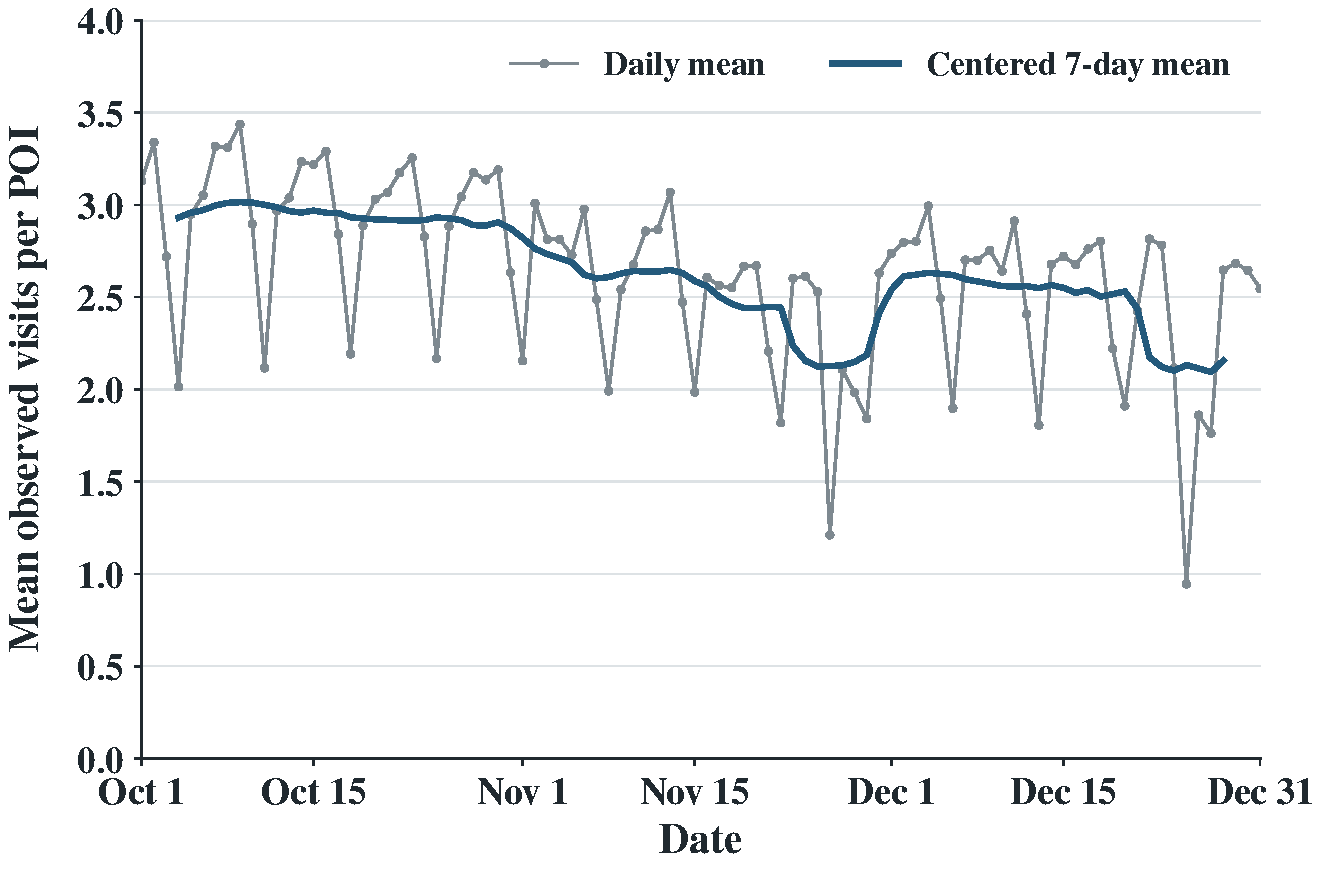
\includegraphics[width=\linewidth]{art/daily_visit.pdf}
    \caption{Daily mean observed visits per POI.}
    \label{fig:daily_visit}
\end{subfigure}
\hfill
\begin{subfigure}[t]{0.49\textwidth}
    \centering
    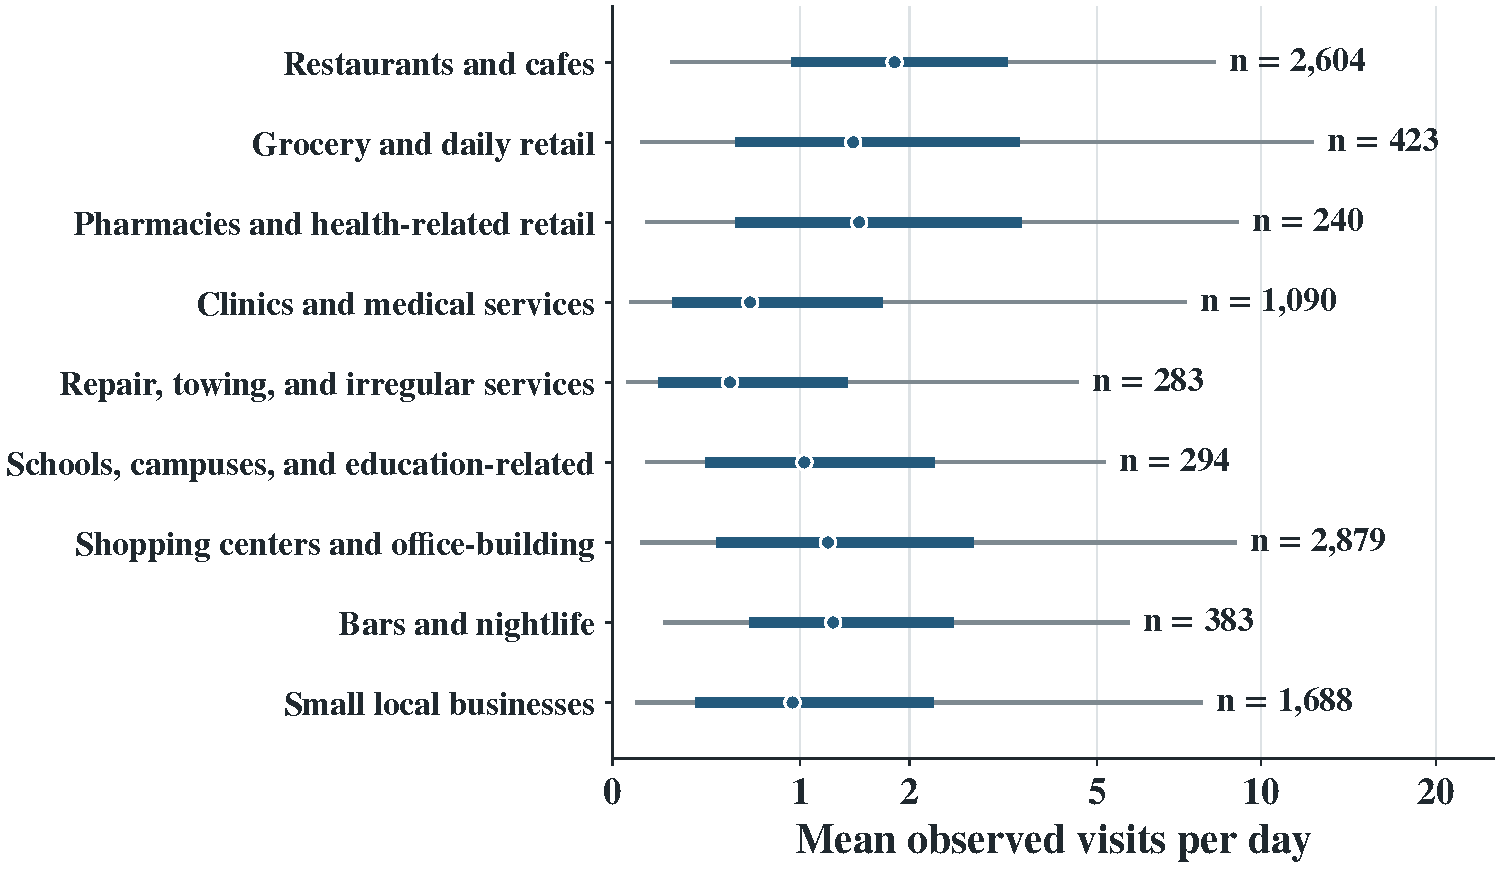
\includegraphics[width=\linewidth]{art/category_visit.pdf}
    \caption{Distribution of mean observed visits across POI categories.}
    \label{fig:category_visit}
\end{subfigure}
\caption{Temporal and category-level characteristics of observed POI visits.}
\label{fig:visit_overview}
\end{figure}

Figure~\ref{fig:visit_overview} summarizes the temporal and category-level variation in observed POI visits.
Panel (a) shows short-term fluctuations and broader temporal changes in aggregate activity, while Panel (b) shows substantial differences in visit levels across the broad POI categories used in the subsequent category-level analysis.

\begin{figure}[!htb]
\centering
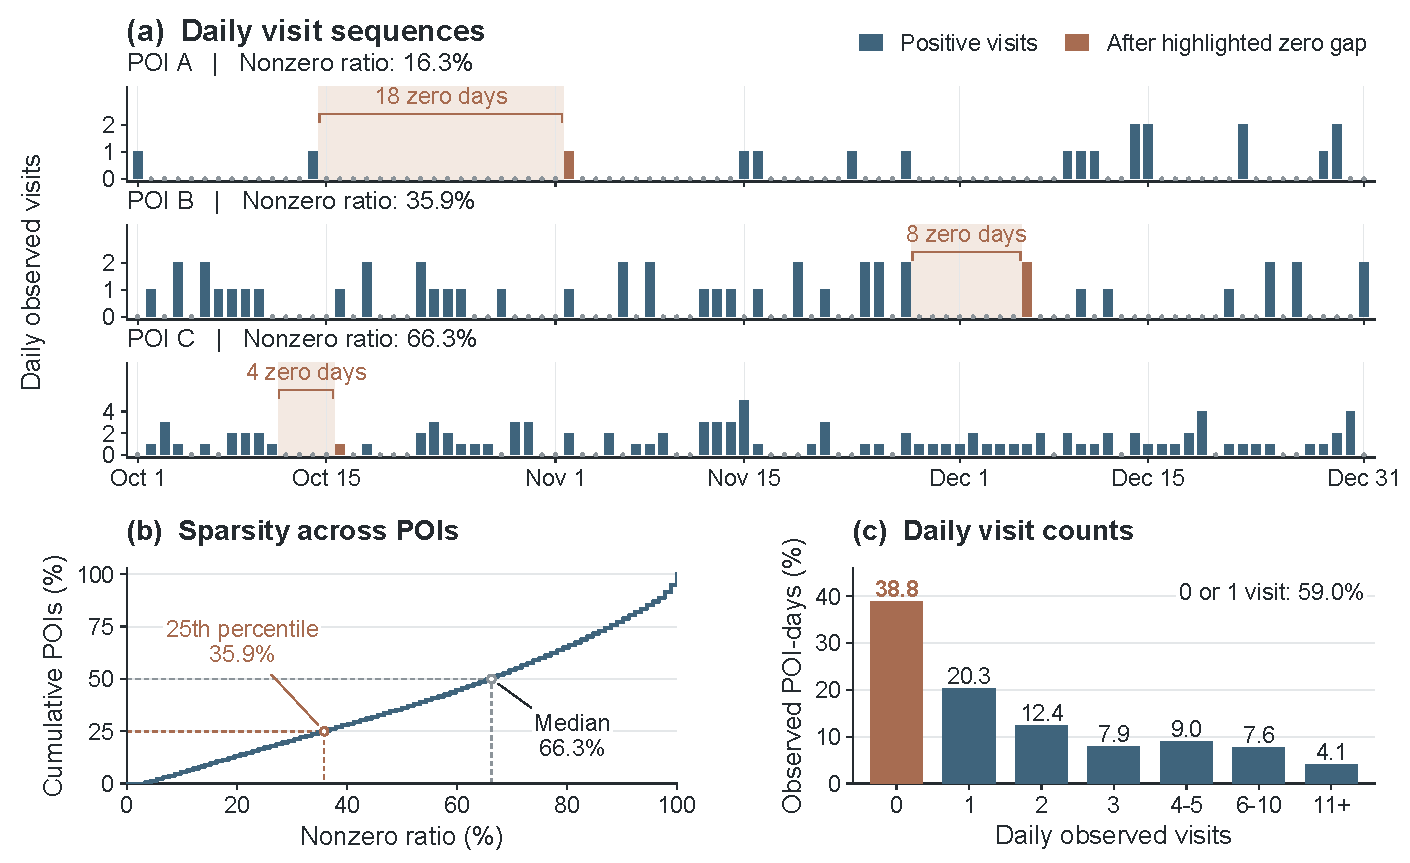
\includegraphics[scale=0.65]{art/poi_temporal_sparsity.pdf}
\caption{Temporal sparsity in POI visit records over the 92-day observation period. (a) Representative daily visit sequences with zero-visit gaps followed by positive visits. (b) Cumulative distribution of POI-level nonzero ratios. (c) Distribution of daily observed visit counts.}
\label{fig:poi_temporal_sparsity}
\end{figure}

Figure~\ref{fig:poi_temporal_sparsity} further shows that POI visits are sparse and intermittent, with prolonged zero-visit periods followed by occasional positive visits.
Across the full observation period, \(38.8\%\) of POI--day observations are zero, and \(59.0\%\) have at most one visit.
The median daily visit count is only \(1\), compared with approximately \(6\), \(9\), and \(22\) visits at the 90th, 95th, and 99th percentiles, respectively.
The maximum daily visit count is substantially larger, producing a long right tail in the visit distribution.
As a result, the data contain a large number of zero or low-count observations together with a much smaller number of high-activity observations.

We then examine POI-level activity to assess whether sparsity is concentrated among particular locations or broadly distributed across POIs.
As shown in Figure~\ref{fig:poi_temporal_sparsity}(b), the median nonzero ratio is \(66.3\%\) over the full observation period, compared with \(35.9\%\) at the 25th percentile.
Over the training period, the corresponding ratios are approximately \(62.5\%\) and \(32.8\%\).
At the lower end of the training-period distribution, \(214\) POIs are active on no more than \(5\%\) of days and \(607\) are active on no more than \(10\%\).
Thus, sparsity varies substantially across POIs rather than being uniformly distributed across the visit matrix.
The amount of self-history, namely a POI's own historical visit information, available for forecasting therefore differs considerably across locations, motivating a separate examination of forecasting performance for POIs with limited historical activity.


\subsection{Prediction Task}
\label{subsec:prediction_task}

We first consider the task of forecasting future daily visits for the \(N\) POIs.
For forecast sample \(b\), the model observes visits over the preceding \(T\) days and predicts visits over the following \(H\) days, where \(T\) is the historical input length and \(H\) is the forecast horizon.
The forecasting problem is therefore multistep, with each model producing an \(H\)-day visit trajectory for every POI.

For sample \(b\), the dynamic features consist of historical visit counts \(X_{b,1,t,j}\), where \(X_{b,1,t,j}\) denotes the observed visit count of POI \(j\) at historical step \(t\), with \(t=1,\ldots,T\) and \(j=1,\ldots,N\).
Across all POIs, these features form the historical visit tensor \(\mathbf{X}_b\in\mathbb{R}^{1\times T\times N}\).
In addition, let \(\mathbf{s}_j\in\mathbb{R}^{D_s}\) denote the encoded static-feature vector of POI \(j\), where \(D_s\) is the number of encoded static-feature dimensions.
For the GNN-static formulation, we replicate \(\mathbf{s}_j\) across the \(T\) input steps and concatenate it with the historical visits along the feature dimension.
The resulting augmented input is \(\widetilde{\mathbf{X}}_b\in\mathbb{R}^{(1+D_s)\times T\times N}\).
The observed and predicted future visits are
\(\mathbf{Y}_b=[Y_{b,h,j}]\) and
\(\hat{\mathbf{Y}}_b=[\hat{Y}_{b,h,j}]\), respectively, with
\(\mathbf{Y}_b,\hat{\mathbf{Y}}_b\in\mathbb{R}^{H\times N}\),
where \(Y_{b,h,j}\) and \(\hat{Y}_{b,h,j}\) denote the observed and predicted visit counts, respectively, for POI \(j\) at forecast horizon \(h\) in sample \(b\), with \(h=1,\ldots,H\) and \(j=1,\ldots,N\).

We vary \(T\) and \(H\) separately to examine two distinct dimensions of forecasting performance.
A longer historical input provides more observations from which the model can learn recurring temporal patterns; for example, a 28-day input contains more weekly cycles than a 14-day input.
A longer forecast horizon instead requires the model to predict further from the observed period, where recent temporal information may become less informative.
We therefore evaluate multiple combinations of \(T\) and \(H\).
We further examine whether forecasting performance differs between POIs with frequent positive historical visits and those with sparse or intermittent visit histories.
Locations with frequent positive visits provide more direct evidence of future activity, whereas sparse or intermittent histories may contain predominantly zero observations.
For such POIs, a model can obtain relatively low aggregate error by repeatedly predicting values close to zero while failing to recover occasional positive visits.
We refer to this behavior as \textit{zero-demand collapse}.
Accordingly, we supplement aggregate forecasting metrics with diagnostics for low-history POIs that separately evaluate positive- and zero-visit observations.


\subsection{Attribution Task}
\label{subsec:attribution_task}

The forecasting task provides the predictive model used to estimate future POI visits, which then serves as the basis for examining what information drives each prediction.
We therefore complement the prediction analysis with an attribution task that distinguishes two sources of predictive information: information transferred from related POIs and information associated directly with the target POI.

\subsubsection{Cross-POI Information}

A target POI may receive information from other locations through geographic proximity, functional similarity, or similarity in historical activity. Such information can supplement limited self-history, especially when the target POI has sparse or irregular observations, but it may also overestimate demand when related POIs exhibit activity that is not realized at the target location. 
We refer to the incorporation of related POIs' historical visit information into the target POI's prediction through graph connections as cross-POI \textit{information transfer}.
For each target POI, forecast horizon, and sample, we consider this transfer \textit{beneficial} when it reduces prediction error compared with using only the target POI's own history, and \textit{harmful} when it increases the error.

To capture dependencies across locations, previous studies have used adjacency matrices to represent geographic proximity, functional similarity, and correlations in historical activity \citep{geng2019spatiotemporal,hajisafi2023learning}. Following this approach, we represent relationships among POIs using an adjacency matrix \(A\in\mathbb{R}^{N\times N}\), where \(A_{ij}\) represents the relationship strength from POI \(i\) to POI \(j\). We consider four types of adjacency matrices. The identity matrix contains only self-connections and serves as a baseline without cross-POI information transfer. Spatial matrices capture geographic proximity through nearest-neighbor connections or distance-based weights. Functional matrices represent similarities among POIs based on shared category labels or industry classifications at different levels of detail. Finally, empirical matrices capture similarities in historical visit patterns through static correlations or correlations updated over rolling historical windows.

Using the adjacency matrices described above, we adopt a graph neural network with adjacency-based information sharing (GNN-adj) formulation, where the model input \(\mathbf{X}_b\in\mathbb{R}^{1\times T\times N}\) contains only historical visit counts, and the selected adjacency matrix \(A\) controls information propagation across POIs. We first compare forecasting performance under different graph structures against the identity-adjacency baseline. Subsequently, we perturb the historical visits of selected groups of connected POIs to examine their influence on target POI predictions, distinguishing \textit{beneficial} transfer, which reduces prediction error relative to the identity-adjacency baseline, from \textit{harmful} transfer, which increases it.


\subsubsection{Target-POI Information}

The second part of the attribution task examines information associated directly with the target POI. In addition to historical visits, each POI has static attributes describing its location, functional identity, brand, parent-place context, and operating conditions. These attributes may help explain why POIs with similar recent visit histories receive different predictions.


To isolate target-POI information from cross-POI propagation, we use the \textit{GNN-static} formulation with the augmented input \(\widetilde{\mathbf{X}}_b\) and identity adjacency, i.e., \(A=I_N\).
Under this setting, each POI's prediction relies on its own historical visits and static attributes rather than information from other POIs.
This formulation supports the subsequent \textit{Feature Attribution and POI Regimes} analysis, where gradient-based attribution is used to quantify the contributions of self-history and static POI attributes to individual predictions.
POIs are then compared according to their attribution profiles to examine whether different locations rely on systematically different sources of predictive information.

To examine how different POI relationships affect forecasting, we use \textit{GNN-adj} in \textit{Alternative Adjacency Matrices}, where the historical visit inputs remain fixed while the adjacency matrix varies.
We also use \textit{GNN-adj} in \textit{Related-POI Perturbation Analysis}, as perturbing the historical visits of connected POIs allows us to examine how information transferred through the graph affects target POI predictions.
In contrast, to identify the contributions of a target POI's own historical visits and static attributes, we use \textit{GNN-static} in \textit{Feature Attribution and POI Regimes}, where identity adjacency excludes cross-POI information transfer and allows attribution analysis to focus on target-specific features.

\section{Methodology}
\label{sec:methodology}

To evaluate POI visit forecasting under different temporal and cross-POI dependencies, we first introduce two temporal graph networks, i.e., EvolveGCN and MTGNN, alongside the benchmark models.
We then describe alternative adjacency matrices and static POI features to represent relationships among POIs and their individual characteristics.
For POIs with sparse visit histories, we introduce additional evaluation metrics to assess whether the models can capture occasional positive visits without overpredicting activity on days with no observed visits.
Finally, we employ related-POI perturbation analysis and gradient-based feature attribution to investigate the sources of cross-POI information transfer and the factors driving individual predictions.

\subsection{Forecasting Models}
\label{subsec:forecasting_models}
\subsubsection{Benchmark Models}
\label{subsubsec:benchmark_models}
To benchmark the forecasting performance of the temporal graph models, we consider three baseline methods with different capacities for capturing temporal patterns: historical average, autoregressive ridge regression (AR-ridge), and long short-term memory (LSTM).

\textit{(1) Historical Average.}
The historical-average predictor uses each POI's mean training-period visits as its forecast.
Let \(\mathcal{T}_{\mathrm{tr}}\) denote the training period and \(y_{\tau,j}\) the observed visits of POI \(j\) on training day \(\tau\).
Its historical average is \(\bar y_j^{\mathrm{hist}}=|\mathcal{T}_{\mathrm{tr}}|^{-1}\sum_{\tau\in\mathcal{T}_{\mathrm{tr}}}y_{\tau,j}\).
The same value is predicted for every test sample and forecast step.
This baseline contains no short-term dynamics but provides a reference for evaluating whether more complex models improve upon typical POI activity levels.

\textit{(2) AR-ridge.}
AR-ridge models the linear relationship between historical visits and future demand.
For POI \(j\), let \(\mathbf v_{b,j}\in\mathbb{R}^{T}\) contain its historical visits in sample \(b\), and let \(\mathbf y_{b,j}\in\mathbb{R}^{H}\) contain its next \(H\) visits.
The model takes the form
\(\mathbf y_{b,j}=B_j^\top\mathbf v_{b,j}+\boldsymbol{\varepsilon}_{b,j}\),
where \(B_j\in\mathbb{R}^{T\times H}\) is the coefficient matrix and \(\boldsymbol{\varepsilon}_{b,j}\) is the error term.
Ridge regularization penalizes large coefficients to reduce estimation instability.
This baseline provides a linear reference for assessing how effectively a POI's own historical visits predict future activity.

\textit{(3) LSTM.}
The LSTM baseline \citep{hochreiter1997long} captures nonlinear temporal dependencies in historical visit sequences.
At historical step \(t\), the model receives the visit vector
\(\mathbf v_{b,t}=(X_{b,1,t,1},\ldots,X_{b,1,t,N})^\top\).
The sequence of \(T\) visit vectors is processed recurrently, and a decoder maps the resulting hidden representation to the \(H\times N\) forecast.
This baseline provides a nonlinear temporal reference without explicitly incorporating graph relationships among POIs.

\subsubsection{EvolveGCN}
\label{subsubsec:evolvegcn}
EvolveGCN is designed for temporal graph data in which the graph-convolution parameters evolve over time \citep{pareja2020evolvegcn}.
A conventional GCN uses a fixed graph-convolution transformation, which can be restrictive when the relevance of cross-node relationships changes across the observed sequence.
EvolveGCN instead updates the graph-convolution parameters recurrently and can therefore operate with either a fixed adjacency matrix or an input-window sequence of adjacency matrices.

In the present application, EvolveGCN serves two purposes.
Under a fixed adjacency matrix, it allows us to compare different prior definitions of POI relationships while holding the forecasting architecture constant.
Under dynamic correlation adjacency, it allows the relationship structure itself to change with recent visitation patterns.
The original EvolveGCN implementation is intended primarily for graph classification or link prediction.
We replace its original output layer with a linear forecasting head that generates continuous \(H\)-step POI visit predictions while retaining its graph-evolution mechanism.

\subsubsection{MTGNN}
\label{subsubsec:mtgnn}

MTGNN combines temporal convolution with graph learning for multivariate time-series forecasting \citep{wu2020connecting}.
A central motivation of MTGNN is that the true dependency structure among variables may not be fully observed in advance.
The model therefore includes an adaptive graph-learning component together with temporal convolutions that capture lagged dependence.

We use the multistep forecasting implementation of MTGNN and initialize it using the alternative graph structures defined below.
This provides a useful contrast with EvolveGCN.
Specifically, EvolveGCN explicitly processes supplied graph information through evolving graph-convolution parameters, whereas MTGNN retains a stronger adaptive graph-learning component.
Differences between the two models are therefore informative not only about predictive performance but also about how strongly the forecasting architecture responds to supplied graph structure.

\subsection{Adjacency Matrices}
\label{subsec:adjacency}

To examine how different relationships among POIs affect forecasting performance, we consider four types of adjacency matrices: \textit{identity adjacency}, \textit{spatial adjacency}, \textit{functional adjacency}, and \textit{visit-correlation adjacency}.

\textit{(1) Identity Adjacency.}
The identity adjacency, \(A=I_N\), contains only self-connections.
It excludes cross-POI information transfer while preserving each POI's own information.

\textit{(2) Spatial Adjacency.}
Spatial relationships are represented using two types of graphs: \(k\)-nearest neighbors (KNN) \citep{cover1967nearest} and radial basis function (RBF) \citep{li2018diffusion}.
The KNN graph connects each POI to its \(k\) geographically nearest locations, representing local spatial relationships through a fixed neighborhood.
The RBF graph instead assigns continuous distance-decay weights,
\(A_{ij}=\exp[-d(i,j)^2/(2\sigma^2)]\),
where \(A_{ij}\) denotes the relationship strength from POI \(i\) to POI \(j\), \(d(i,j)\) is their geographic distance, and \(\sigma\) controls the rate at which the relationship weakens with distance.

\textit{(3) Functional Adjacency.}
Functional relationships are represented using top category, sub-category, NAICS-2, and NAICS-4.
For each classification \(q\in\{\mathrm{cat},\mathrm{subcat},\mathrm{naics2},\mathrm{naics4}\}\), the corresponding adjacency matrix is defined as
\(
A_{ij}^{(q)}=\mathbb{I}\{q_i=q_j\},
\)
where \(q_i\) and \(q_j\) denote the classification labels or industry-code prefixes of POIs \(i\) and \(j\), respectively, and \(\mathbb{I}\{\cdot\}\) is the indicator function, equal to one when the condition holds and zero otherwise.
Top category and NAICS-2 represent broader functional groups, whereas sub-category and NAICS-4 represent more specific classifications.

\textit{(4) Visit-Correlation Adjacency.}
Historical similarity is represented using Pearson correlations between POI visit sequences.
Specifically, the correlation between POIs \(i\) and \(j\) is computed as
\(\rho_{ij}=\operatorname{corr}((y_{\tau,i})_{\tau\in\mathcal{T}_{\mathrm{tr}}},(y_{\tau,j})_{\tau\in\mathcal{T}_{\mathrm{tr}}})\),
where \(\operatorname{corr}(\cdot,\cdot)\) denotes the Pearson correlation coefficient computed from the daily visit counts of the two POIs over the training period.
For the static correlation graph, the adjacency weights are defined as
\(A_{ij}=|\rho_{ij}|\mathbb{I}\{|\rho_{ij}|\geq\eta_c\}\),
where \(\eta_c\) is the threshold used to remove weak correlations.
To capture changes in visit-pattern similarity over time, we additionally construct dynamic adjacency matrices for EvolveGCN using rolling historical windows.
Specifically, for a rolling window of \(w\) historical steps ending at \(t\), the correlation is computed as
\(\rho_{ij}^{(b,t)}=\operatorname{corr}((X_{b,1,\tau,i})_{\tau=t-w+1}^{t},(X_{b,1,\tau,j})_{\tau=t-w+1}^{t})\),
where \(w\) is the rolling-window length.
At each time step, the dynamic adjacency connects each POI to its \(k\) most strongly correlated neighbors based on \(|\rho_{ij}^{(b,t)}|\), using these absolute correlations as edge weights.

\subsection{Forecast Evaluation}
\label{subsec:low_history_method}

We evaluate the forecasting models from three perspectives: \textit{overall forecasting accuracy}, \textit{visit-density sensitivity}, and \textit{low-history POI evaluation}.

\textit{(1) Overall Forecasting Accuracy.}
We evaluate forecasting accuracy using mean absolute error (MAE), root mean squared error (RMSE), relative squared error (RSE), and Pearson correlation (CORR).
MAE and RMSE measure prediction errors, while RSE is the square root of the ratio of summed squared errors to summed squared deviations from the observed mean at each forecast horizon.
CORR measures the Pearson correlation between observed and predicted visits, while anomaly correlation measures their correlation after subtracting each POI's historical average \(\bar y_j^{\mathrm{hist}}\).
All metrics are computed across test samples and POIs for each forecast horizon.

\textit{(2) Visit-Density Sensitivity.}
To examine how historical visit sparsity affects forecasting performance, we construct POI subsets with progressively higher frequencies of positive visits.
For POI \(j\), the training-period nonzero ratio is defined as
\(
r_j=
\frac{1}{|\mathcal{T}_{\mathrm{tr}}|}
\sum_{\tau\in\mathcal{T}_{\mathrm{tr}}}
\mathbb{I}\{y_{\tau,j}>0\}.
\)
We consider three approaches to constructing these subsets.
The \textit{density-based} approach ranks POIs by their training-period nonzero ratios \(r_j\).
The \textit{recent-density} approach ranks POIs by their nonzero ratios over the final \(L_{\mathrm{rec}}\) days of the training period, where \(L_{\mathrm{rec}}\) denotes the recent-history window length.
The \textit{persistence-density} approach combines the overall nonzero ratio with the probability of consecutive positive-visit days, estimated as \(p_j^{\mathrm{persist}}=\frac{\sum_{\tau\in\mathcal{T}_{\mathrm{tr}}^{-}}\mathbb{I}\{y_{\tau,j}>0,\;y_{\tau+1,j}>0\}}{\sum_{\tau\in\mathcal{T}_{\mathrm{tr}}^{-}}\mathbb{I}\{y_{\tau,j}>0\}}\), where \(\mathcal{T}_{\mathrm{tr}}^{-}\) contains all training days except the last day.
For each approach, we retain POIs whose ranking scores exceed the corresponding quantile threshold, denoted by \(\gamma^{\mathrm{den}},\gamma^{\mathrm{rec}},\gamma^{\mathrm{per}}\in(0,1)\), respectively.
We consider quantile thresholds of \(0.10\), \(0.25\), \(0.50\), and \(0.75\), corresponding to the percentages of POIs excluded from each subset.
For example, Dense10 retains the top \(90\%\) of POIs ranked by their training-period nonzero ratios.
The same suffix convention applies to the recent-density and persistence-density subsets.
For each subset, we reconstruct the visit matrix and retrain the forecasting model.

\textit{(3) Low-History POI Evaluation.}
To assess forecasting performance for POIs with sparse historical activity, we identify locations characterized by frequent zero observations and low average visit counts.
The low-history POI set is defined as
\(\mathcal{I}_{0}=\left\{j:z_j\geq\eta_z,\;0<\bar y_j^{\mathrm{hist}}\leq Q_{\alpha}\right\}\),
where \(z_j=1-r_j\) denotes the training-period zero-visit ratio, and \(Q_{\alpha}\) is the \(\alpha\)-quantile of positive historical averages across POIs.
For these POIs, we distinguish test events with positive observed visits from those with zero observed visits, defined respectively as
\(\Omega_0^+=\{(b,h,j):j\in\mathcal{I}_0,\;Y_{b,h,j}>0\}\)
and
\(\Omega_0^0=\{(b,h,j):j\in\mathcal{I}_0,\;Y_{b,h,j}=0\}\).
We use three diagnostic metrics to characterize model predictions for these events.

\textit{(i) Prediction Lift.}
Lift measures the average increase in predicted visits relative to the historical-average (HA) baseline, 
i.e.,
\(\mathrm{Lift}=\frac{\sum_{(b,h,j)\in\Omega_0^+\cup\Omega_0^0}(\max\{0,\hat Y_{b,h,j}\}-\bar y_j^{\mathrm{hist}})}{|\Omega_0^+|+|\Omega_0^0|}\).

\textit{(ii) Demand Mass Recovery Ratio (DMR).}
DMR measures the ratio of predicted to observed visit totals among events with positive realized demand,
i.e., 
\(\mathrm{DMR}^{\mathrm{model}}=\frac{\sum_{(b,h,j)\in\Omega_0^+}\hat Y_{b,h,j}}{\sum_{(b,h,j)\in\Omega_0^+}Y_{b,h,j}}\),
while the corresponding HA baseline is
\(\mathrm{DMR}^{\mathrm{HA}}=\frac{\sum_{(b,h,j)\in\Omega_0^+}\bar y_j^{\mathrm{hist}}}{\sum_{(b,h,j)\in\Omega_0^+}Y_{b,h,j}}\).
The difference
\(\Delta\mathrm{DMR}=\mathrm{DMR}^{\mathrm{model}}-\mathrm{DMR}^{\mathrm{HA}}\)
measures the change in predicted demand mass relative to the HA baseline.

\textit{(iii) False Activation Rate (FAR).}
FAR measures the proportion of zero-visit events for which the predicted visit count reaches a specified threshold.
For an activation threshold \(\eta_{\mathrm{FAR}}>0\), we define
\(\mathrm{FAR}_{\eta_{\mathrm{FAR}}}=\frac{1}{|\Omega_0^0|}\sum_{(b,h,j)\in\Omega_0^0}\mathbb{I}\{\hat Y_{b,h,j}\geq\eta_{\mathrm{FAR}}\}\).

\subsection{Related-POI Perturbation Analysis}
\label{subsec:perturbation_method}

Building on the low-history POI evaluation, we further examine how information transferred from related POIs affects individual predictions.
We first identify \textit{graph-transfer regimes} based on graph lift and historical activity at the target and neighboring POIs, and then conduct \textit{neighbor-group perturbation} to identify which neighbors contribute to the observed prediction changes.

\textit{(1) Graph-Transfer Regimes.}
We characterize cross-POI information transfer by comparing predictions from the same forecasting architecture under different adjacency matrices.
For test sample \(b\), forecast horizon \(h\), and target POI \(j\), let \(\hat Y_{b,h,j}^{A}\) denote the prediction under a non-identity adjacency matrix \(A\), and \(\hat Y_{b,h,j}^{\mathrm{ID}}\) the corresponding prediction under identity adjacency.
Their difference, defined as
\(G_{b,h,j}=\hat Y_{b,h,j}^{A}-\hat Y_{b,h,j}^{\mathrm{ID}}\),
measures the change in predicted visits associated with cross-POI information transfer, which we refer to as \textit{graph lift}.

For low-history POIs \(j\in\mathcal{I}_0\), we characterize graph transfer using the historical activity of the target POI and its connected neighbors.
Let \(\mathcal{N}(j)=\{i\neq j:A_{ij}>0\}\) denote the neighbors of POI \(j\) under the selected adjacency matrix.
We define \textit{target evidence} as the target POI's average historical visits,
\(\frac{1}{T}\sum_{t=1}^{T}X_{b,1,t,j}\),
and \textit{neighbor evidence} as the average historical visits across its connected neighbors,
\(\frac{1}{T|\mathcal{N}(j)|}\sum_{i\in\mathcal{N}(j)}\sum_{t=1}^{T}X_{b,1,t,i}\),
for POIs with nonempty neighborhoods.
Under functional adjacency, neighbor evidence summarizes historical activity among POIs sharing the corresponding functional classification.

We classify prediction events according to target evidence, neighbor evidence, graph lift, and realized visits.
Low and high levels of target and neighbor evidence are determined using their respective empirical medians among low-history events.
Positive graph lift is defined by \(G_{b,h,j}\geq\eta_G\), where \(\eta_G>0\) is the graph-lift threshold.
Positive activation follows the threshold \(\eta_{\mathrm{FAR}}\) defined in the preceding subsection.
Table~\ref{tab:graph_transfer_regime_definitions} summarizes the resulting graph-transfer regimes.

\begin{table}[t]
\centering
\begin{adjustbox}{max width=\textwidth}
\begin{tabular}{lll}
\toprule
Regime & Definition & Interpretation \\
\midrule
Substitutive transfer
& Low target evidence, high neighbor evidence, positive graph lift
& Neighbor activity supplements limited target history. \\
Spurious transfer
& Substitutive transfer with \(Y_{b,h,j}=0\) and positive activation
& Neighbor information raises predictions for zero-visit events. \\
Confirmatory transfer
& High target evidence, high neighbor evidence, positive graph lift
& Neighbor activity reinforces target-history information. \\
Redundant self-history
& High target evidence, small or negative graph lift
& Predictions rely primarily on target-history information. \\
Conservative zero
& \(Y_{b,h,j}=0\) and no positive activation
& The model maintains low predictions for zero-visit events. \\
\bottomrule
\end{tabular}
\end{adjustbox}
\caption{Graph-transfer regime definitions for low-history POIs.}
\label{tab:graph_transfer_regime_definitions}
\end{table}

To assess the predictive value of graph transfer, we compute the event-level MAE gain as
\(|Y_{b,h,j}-\hat Y_{b,h,j}^{\mathrm{ID}}|-|Y_{b,h,j}-\hat Y_{b,h,j}^{A}|\).
Positive values indicate lower prediction error under non-identity adjacency, whereas negative values indicate higher error.
We compare graph lift and MAE gain across the identified regimes to characterize the conditions under which cross-POI information improves or worsens forecasting accuracy.

\textit{(2) Neighbor-Group Perturbation.}
We further examine which neighboring POIs contribute to the graph-transfer effects identified above.
For each target POI \(j\), we select a group \(S\subseteq\mathcal{N}(j)\) and perturb its historical visit inputs while keeping the forecasting model and adjacency matrix fixed.
Let \(\mathbf{X}_b^{(-S)}\) denote the input obtained by setting the historical visits of POIs in \(S\) to zero while leaving all other inputs unchanged.
The perturbation effect is defined as
\begin{equation}
D_{b,h,j}(S)
=
\hat Y_{b,h,j}^{A}(\mathbf{X}_b)
-
\hat Y_{b,h,j}^{A}(\mathbf{X}_b^{(-S)}),
\label{eq:perturbation_effect}
\end{equation}
where a positive value indicates that the selected neighbor group increases the target POI's original prediction.

We consider several neighbor groups to examine different sources of information transfer.
Perturbing all neighbors measures the overall neighborhood effect, while perturbing recently active neighbors examines the contribution of recent activity.
High-mean and low-mean neighbors are distinguished by their average historical visits, and the top-10 active neighbors are selected to examine whether graph transfer is concentrated among highly active locations.
Randomly selected neighbors provide a reference for comparison.
We additionally perturb highly correlated neighbors and temporally aligned neighbors to examine the contributions of similar visit patterns.
For each group, we compare perturbation effects across beneficial and harmful graph-transfer events and evaluate the associated changes in prediction error, positive-demand recovery, and false activation.

\subsection{Feature Attribution and POI Regimes}
\label{subsec:attribution_method}

The preceding analysis examines the influence of information transferred through graph connections.
We next investigate the contributions of a target POI's own historical visits and static attributes using the GNN-static formulation introduced in Section~\ref{subsec:attribution_task}.
With identity adjacency excluding cross-POI propagation, we apply gradient-based attribution to individual predictions and examine how the resulting information sources vary across POIs.

\textit{(1) Gradient-Based Feature Attribution.}
We use Gradient \(\times\) Input to quantify the contribution of each input component to an individual prediction.
Let \(x_{b,j,m}\) denote the \(m\)-th input component of POI \(j\) in the augmented input \(\widetilde{\mathbf{X}}_b\), including its historical visits and encoded static attributes.
The attribution score for forecast horizon \(h\) is defined as
\(\phi_{b,h,j,m}=x_{b,j,m}\frac{\partial\hat Y_{b,h,j}}{\partial x_{b,j,m}}\).
The score combines the input value with the local sensitivity of the prediction to that input.

To summarize attribution across different information sources, we consider five feature groups: \textit{history}, \textit{location}, \textit{identity}, \textit{parent}, and \textit{others}.
History includes historical visit counts; location includes latitude and longitude; identity includes category, industry, and brand information; parent includes parent-place information; and others includes opening-hour features and their missingness indicators.
Let \(\mathcal{G}\) denote the set of these groups and \(\mathcal{F}_g\) the input components belonging to group \(g\in\mathcal{G}\).
For each POI \(j\), we aggregate the absolute attribution scores across test samples and forecast horizons and compute the normalized attribution share as
\begin{equation}
\pi_{j,g}
=
\frac{
\sum_{b,h}
\sum_{m\in\mathcal{F}_g}
|\phi_{b,h,j,m}|
}{
\sum_{g'\in\mathcal{G}}
\sum_{b,h}
\sum_{m\in\mathcal{F}_{g'}}
|\phi_{b,h,j,m}|
}.
\label{eq:attribution_group_share}
\end{equation}
The resulting attribution profile
\(\boldsymbol{\pi}_j=(\pi_{j,g})_{g\in\mathcal{G}}\)
summarizes the relative contributions of different information sources to predictions for POI \(j\).

\textit{(2) Attribution-Based POI Regimes.}
We characterize differences in feature reliance by standardizing the attribution shares across POIs.
For each feature group \(g\in\mathcal{G}\), let \(\mu_g\) and \(\sigma_g\) denote the mean and standard deviation of \(\pi_{j,g}\) across POIs, respectively.
The standardized attribution score is defined as
\begin{equation}
\widetilde{\pi}_{j,g}
=
\frac{\pi_{j,g}-\mu_g}{\sigma_g}.
\end{equation}
Each POI is assigned to the regime corresponding to its highest standardized attribution score.
The resulting five regimes are history-driven, location-driven, identity-driven, parent-driven, and others-driven.
These assignments reflect relative feature reliance across POIs rather than the largest original attribution share.
We further compare forecasting errors across the resulting regimes.

\textit{(3) Parent-Place Attribution.}
To examine the role of containment relationships in POI predictions, we focus on locations with valid parent-place information.
For each embedded POI, we compare the parent-place attribution share \(\pi_{j,\mathrm{parent}}\) with the combined share of the remaining information sources, \(1-\pi_{j,\mathrm{parent}}\).
We then aggregate these shares across different embedded POI groups to assess how reliance on parent-place context varies with POI function and surrounding destination type.

\textit{(4) Semantic Granularity.}
We further examine how category and industry representations at different levels of granularity contribute to individual predictions.
Using MTGNN with identity adjacency, we compare the attribution of four semantic descriptors: top category, sub-category, NAICS-2, and NAICS-4.
For each prediction event, we compute the Gradient \(\times\) Input attribution scores associated with each descriptor and compare their relative contributions.
We report the average attribution share of each descriptor, its dominance rate among the four semantic representations, and the MAE of prediction events in which it is dominant.
These measures characterize both the relative influence of semantic information and the forecasting accuracy associated with different dominant descriptors.

\section{Empirical Results}
\label{sec:results}

Figure~\ref{fig:exp_logic} outlines the empirical analyses, organized into prediction and attribution tasks.
We begin in Section~\ref{subsec:forecasting_results} by comparing forecasting performance across historical input lengths and forecast horizons, examining visit-history sparsity, and evaluating positive-demand recovery and false activation for low-history POIs.
To investigate information sharing among POIs, Section~\ref{subsec:information_sharing_results} compares alternative adjacency matrices and examines how related-POI perturbation affects individual forecasts.
Finally, Section~\ref{subsec:explanation_results} analyzes attribution patterns and POI attribution regimes to identify the information sources driving predictions, while examining parent-place context and semantic granularity to assess their roles in forecasting.

\begin{figure}[htbp]
\centering
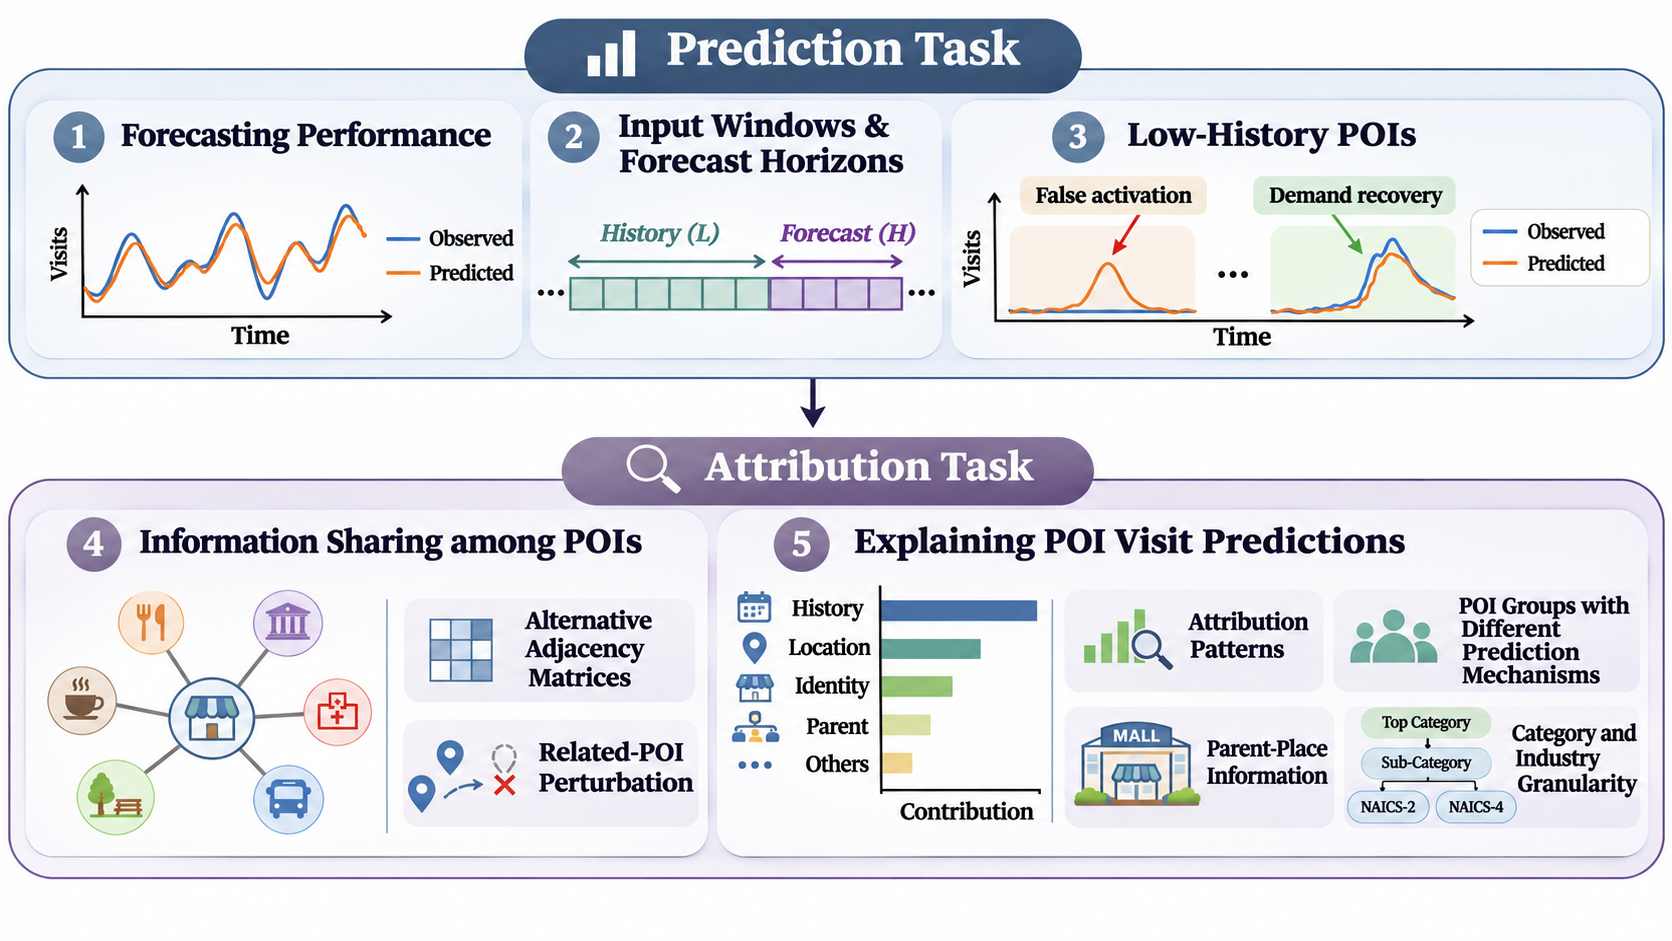
\includegraphics[scale=0.23]{art/exp_logic.png}
\caption{Design logic of the empirical analyses.}
\label{fig:exp_logic}
\end{figure}

\subsection{Parameter Settings}
\label{subsec:parameter_settings}

We first evaluate the forecasting models across four combinations of historical input lengths and forecast horizons. The observations are divided chronologically into training, validation, and test periods, and model configurations are selected based on validation loss. The subsequent analyses use \(T=28\), \(H=14\) for density sensitivity, graph transfer, and neighbor perturbation, providing a longer historical window to characterize POI activity and cross-POI relationships. In contrast, demand recovery and feature attribution use \(T=14\), \(H=7\) to focus on near-term predictions, particularly the recovery of intermittent positive visits and the contributions of recent inputs.
Table~\ref{tab:parameter_settings} summarizes the main experimental settings.

\begin{table}[!htbp]
\centering
\fontsize{9pt}{11pt}\selectfont
\caption{Parameter settings for POI visit forecasting and attribution.}
\label{tab:parameter_settings}
\setlength{\tabcolsep}{5pt}
\renewcommand{\arraystretch}{1.12}
\begin{tabularx}{\linewidth}{@{}
>{\raggedright\arraybackslash}p{0.34\linewidth}
>{\raggedright\arraybackslash}X@{}}
\toprule
Parameter & Value \\
\midrule
Training / validation / test
& Oct.~1--Nov.~26 / Nov.~27--Dec.~3 /
Dec.~4--31, 2020 \\

\addlinespace[2pt]
KNN neighbors \(k\)
& 10 \\

RBF bandwidth \(\sigma\) and cutoff
& 1 km and 2 km \\

Visit-correlation threshold \(\eta_c\)
& 0.30 \\

\addlinespace[2pt]
Ridge penalty
& 100 \\

Hidden dimensions
& EvolveGCN: 32;
GNN-static: 32;
LSTM: 128 \\

Learning rate (EvolveGCN, NAICS-2)
& \(5\times10^{-4}\) \\

Batch sizes
& EvolveGCN: 6;
GNN-static: 6;
LSTM: 32;
MTGNN: 4 \\

\addlinespace[2pt]
Recent-density window \(L_{\mathrm{rec}}\)
& 14 days \\

Density exclusion quantiles
& \(\{0.10,0.25,0.50,0.75\}\) \\

Low-history thresholds
& \(\eta_z=0.70\), \(\alpha=0.25\) \\

Graph-lift threshold \(\eta_G\)
& 0.1 \\

False-activation threshold \(\eta_{\mathrm{FAR}}\)
& 0.5 \\

Static-feature dimensions \(D_s\)
& 52 \\
\bottomrule
\end{tabularx}
\end{table}

\subsection{Forecasting Performance}
\label{subsec:forecasting_results}


\subsubsection{Input Windows and Forecast Horizons}
\label{subsubsec:multi_horizon_results}

To provide a reliable predictive foundation for the subsequent attribution analysis, we first compare the temporal graph models with the historical-average, AR-ridge, and LSTM benchmarks across different input lengths and forecast horizons.
Specifically, we evaluate \((T,H)\in\{(14,7),(28,7),(28,14),(28,28)\}\) to examine how forecasting performance varies with the amount of historical information and the prediction horizon.
Comparing the first two settings isolates the effect of extending the input history from 14 to 28 days, while the remaining settings examine forecast horizons of 7, 14, and 28 days with \(T=28\).


\begin{table}[!htbp]
\centering
\begingroup
\singlespacing
\fontsize{9pt}{10pt}\selectfont
\setlength{\tabcolsep}{3pt}
\renewcommand{\arraystretch}{0.92}
\captionsetup{skip=4pt}
\caption{Multi-horizon forecasting diagnostics. For each \((T,H)\), the best MTGNN and non-identity EvolveGCN adjacencies are selected by validation loss. Skill is \(100(1-\mathrm{MAE}_{\mathrm{model}}/\mathrm{MAE}_{\mathrm{HA}})\). Anomaly correlation uses deviations from the historical average.}
\label{tab:multihorizon}
\begin{adjustbox}{max width=\linewidth}
\begin{tabular}{lllrrrrrrr}
\toprule
\((T,H)\) & Model & Adjacency & MAE & RSE & CORR &
Skill (\%) & Anom. CORR & \(\Delta\mathrm{DMR}\) &
\(\mathrm{FAR}_{0.5}\) \\
\midrule
(14,7) & Historical average & -- & 1.47 & 0.45 & 0.90 & 0.00 & -- & 0.00 & 0.00 \\
(14,7) & AR-ridge & -- & 1.43 & 0.47 & 0.88 & 2.63 & 0.40 & -0.00 & 0.01 \\
(14,7) & LSTM & -- & 1.86 & 0.97 & 0.35 & -26.05 & 0.24 & -0.00 & 0.00 \\
(14,7) & MTGNN & NAICS-2 & 1.22 & 0.37 & 0.93 & 17.34 & 0.58 & -0.09 & 0.01 \\
(14,7) & EvolveGCN & Identity & 1.37 & 0.45 & 0.89 & 7.01 & 0.38 & 0.19 & 0.18 \\
(14,7) & EvolveGCN & Distance RBF & 1.40 & 0.45 & 0.89 & 4.82 & 0.37 & 0.19 & 0.26 \\
\midrule
(28,7) & Historical average & -- & 1.48 & 0.45 & 0.90 & 0.00 & -- & 0.00 & 0.00 \\
(28,7) & AR-ridge & -- & 1.66 & 0.82 & 0.65 & -12.50 & 0.15 & -0.00 & 0.02 \\
(28,7) & LSTM & -- & 1.98 & 0.99 & 0.29 & -33.87 & 0.24 & -0.00 & 0.02 \\
(28,7) & MTGNN & Identity & 1.20 & 0.37 & 0.93 & 18.79 & 0.58 & -0.13 & 0.01 \\
(28,7) & EvolveGCN & Identity & 1.38 & 0.46 & 0.89 & 6.75 & 0.37 & 0.13 & 0.13 \\
(28,7) & EvolveGCN & Distance RBF & 1.41 & 0.46 & 0.89 & 4.88 & 0.37 & 0.08 & 0.15 \\
\midrule
(28,14) & Historical average & -- & 1.47 & 0.44 & 0.90 & 0.00 & -- & 0.00 & 0.00 \\
(28,14) & AR-ridge & -- & 1.61 & 0.74 & 0.70 & -9.76 & 0.19 & 0.00 & 0.03 \\
(28,14) & LSTM & -- & 2.00 & 1.00 & 0.28 & -36.16 & 0.23 & 0.00 & 0.03 \\
(28,14) & MTGNN & NAICS-2 & 1.20 & 0.36 & 0.94 & 17.93 & 0.59 & -0.11 & 0.01 \\
(28,14) & EvolveGCN & Identity & 1.40 & 0.47 & 0.89 & 4.62 & 0.33 & 0.15 & 0.19 \\
(28,14) & EvolveGCN & Distance RBF & 1.45 & 0.48 & 0.88 & 0.90 & 0.32 & 0.09 & 0.16 \\
\midrule
(28,28) & Historical average & -- & 1.47 & 0.44 & 0.91 & 0.00 & -- & 0.00 & 0.00 \\
(28,28) & AR-ridge & -- & 1.54 & 0.62 & 0.79 & -4.54 & 0.29 & 0.01 & 0.06 \\
(28,28) & LSTM & -- & 2.01 & 1.00 & 0.28 & -36.64 & 0.22 & 0.01 & 0.06 \\
(28,28) & MTGNN & Top category & 1.27 & 0.41 & 0.93 & 13.72 & 0.49 & -0.10 & 0.00 \\
(28,28) & EvolveGCN & Identity & 1.45 & 0.49 & 0.88 & 1.37 & 0.26 & 0.14 & 0.21 \\
(28,28) & EvolveGCN & Distance RBF & 1.47 & 0.50 & 0.88 & -0.24 & 0.26 & 0.09 & 0.20 \\
\bottomrule
\end{tabular}
\end{adjustbox}
\endgroup
\end{table}


Table~\ref{tab:multihorizon} compares the forecasting performance of the benchmark and temporal graph models across the four settings.
MTGNN achieves the lowest test MAE and highest CORR and anomaly correlation in every setting, with MAE skill relative to the historical average ranging from \(13.72\%\) to \(18.79\%\).
Within EvolveGCN, identity adjacency consistently outperforms the validation-selected non-identity adjacency, indicating that incorporating cross-POI connections does not necessarily improve aggregate forecasting accuracy.
The historical average remains a competitive POI-specific baseline, particularly at longer horizons.
At \((T,H)=(28,28)\), for example, EvolveGCN with distance RBF adjacency has slightly negative MAE skill relative to the historical average.
AR-ridge improves upon the historical average at \((14,7)\) but performs worse with longer input windows, while LSTM has higher MAE than both the historical average and EvolveGCN across all four settings.

The comparison also reveals different sensitivities to input length.
At \(H=7\), doubling the input history has little effect on EvolveGCN with identity adjacency: its MAE changes from \(1.37\) to \(1.38\), and its MAE skill changes from \(7.01\%\) to \(6.75\%\).
In contrast, AR-ridge MAE increases from \(1.43\) to \(1.66\), with RSE increasing from \(0.47\) to \(0.82\).
These results indicate that additional historical observations do not uniformly improve forecasting performance.

\begin{figure}[!htb]
\centering
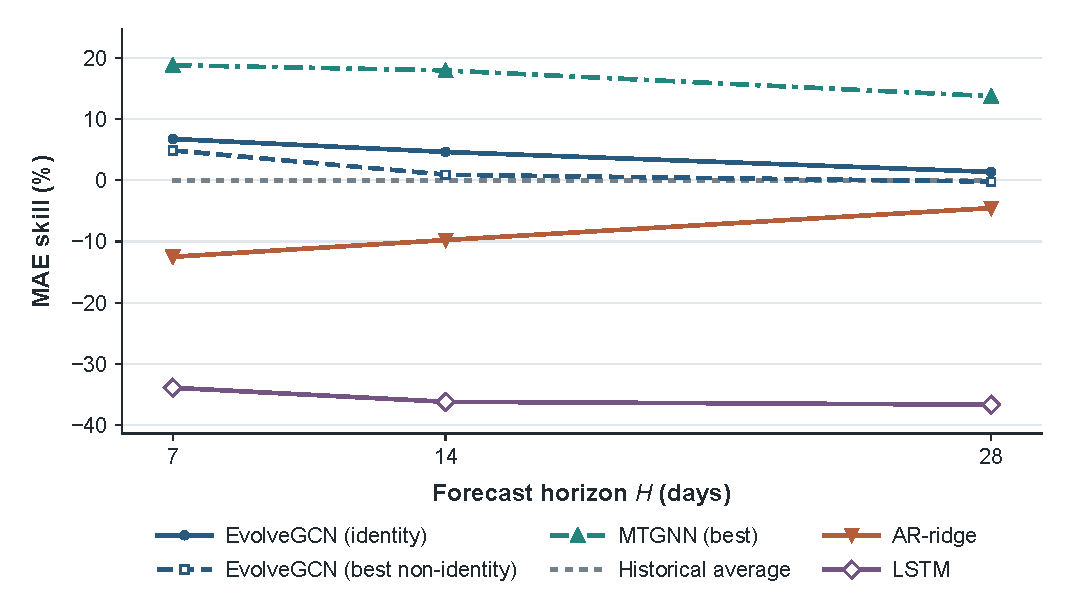
\includegraphics[scale=0.60]{art/forecasting_performance_across_horizons.pdf}
\caption{Mean absolute error (MAE) skill relative to the historical average at \(T=28\) days. The best MTGNN and non-identity EvolveGCN configurations are selected by validation loss within each horizon. The 28-day horizon has one test forecast origin.}
\label{fig:forecast_horizon_skill}
\end{figure}

To further examine the effect of forecast horizon, Figure~\ref{fig:forecast_horizon_skill} illustrates how MAE skill relative to the historical average changes as \(H\) increases with \(T=28\).
For EvolveGCN with identity adjacency, MAE skill decreases from \(6.75\%\) at \(H=7\) to \(4.62\%\) at \(H=14\) and \(1.37\%\) at \(H=28\).
The corresponding values for the validation-selected MTGNN configurations are \(18.79\%\), \(17.93\%\), and \(13.72\%\).
Both architectures maintain an advantage over the historical average, although this advantage diminishes at longer horizons, particularly for EvolveGCN.
At \(H=28\), where the evaluation contains only one test forecast origin, EvolveGCN with identity adjacency retains a CORR of \(0.88\), while its anomaly correlation declines from \(0.37\) at \(H=7\) to \(0.26\).
This suggests that EvolveGCN maintains relatively strong agreement with overall visit levels but becomes less effective at capturing deviations from the historical average as the forecast horizon increases.

Despite its superior aggregate forecasting accuracy, MTGNN does not consistently achieve better positive-demand recovery among low-history POIs.
As shown in Table~\ref{tab:multihorizon}, at \((T,H)=(28,14)\), MTGNN achieves a \(\Delta\mathrm{DMR}\) of \(-0.11\) and a \(\mathrm{FAR}_{0.5}\) of \(0.01\), whereas EvolveGCN with identity adjacency achieves a \(\Delta\mathrm{DMR}\) of \(0.15\) and a \(\mathrm{FAR}_{0.5}\) of \(0.19\).
This contrast indicates that lower aggregate forecasting error does not necessarily correspond to greater positive-demand recovery for POIs with sparse histories, while increased recovery may be accompanied by more false activations.
We examine this tradeoff in greater detail in the following analysis of low-history POIs.






\subsubsection{Low-History POIs}
\label{subsubsec:low_history_results}


As discussed in Section~\ref{subsec:data}, POI visit records contain frequent zero observations, and the degree of sparsity varies across locations.
This motivates us to examine how historical visit sparsity affects forecasting performance, particularly whether models can capture occasional positive visits from limited historical information.
We first compare forecasting performance across POI subsets with progressively higher visit densities to assess how model accuracy varies as sparse POIs are excluded.
We then focus on low-history POIs to evaluate positive-demand recovery and false activations on zero-visit events.


\textit{(1) Density Sensitivity.}
For the density sensitivity analysis, we construct three types of subsets based on different measures of historical activity.
The density-based subsets retain locations with the largest overall training-period nonzero ratios.
The recent-density subsets emphasize activity near the end of the training period, while the persistence-density subsets favor locations with frequent activity on consecutive days.
We rebuild the visit matrix and refit EvolveGCN with identity adjacency for each subset at \(T=28\), \(H=14\).

\begin{table}[!htbp]
\centering
\footnotesize
\caption{Visit-density sensitivity at \(T=28\), \(H=14\). Skill is relative to the historical average within each subset.}
\label{tab:sublevel}
\begingroup
\setlength{\tabcolsep}{4pt}
\renewcommand{\arraystretch}{1.1}
\begin{tabular*}{\linewidth}{@{\extracolsep{\fill}}lccccccc@{}}
\toprule
\makecell[l]{Subset}
& \makecell[c]{POIs}
& \makecell[c]{Nonzero\\ratio}
& \makecell[c]{EvolveGCN\\MAE}
& \makecell[c]{HA\\MAE}
& \makecell[c]{Skill\\(\%)}
& \makecell[c]{RSE}
& \makecell[c]{CORR} \\
\midrule
Full & 9,884 & 0.62 & 1.40 & 1.47 & 4.62 & 0.47 & 0.89 \\
Dense10 & 8,896 & 0.68 & 1.52 & 1.61 & 5.54 & 0.47 & 0.89 \\
Dense25 & 7,413 & 0.76 & 1.71 & 1.83 & 6.42 & 0.47 & 0.88 \\
Dense50 & 4,942 & 0.88 & 2.14 & 2.31 & 7.44 & 0.47 & 0.88 \\
Dense75 & 2,471 & 0.97 & 2.92 & 3.16 & 7.86 & 0.46 & 0.89 \\
Recent-dense10 & 8,896 & 0.68 & 1.52 & 1.60 & 5.14 & 0.47 & 0.89 \\
Recent-dense25 & 7,413 & 0.76 & 1.71 & 1.82 & 5.85 & 0.47 & 0.88 \\
Recent-dense50 & 4,942 & 0.86 & 2.13 & 2.27 & 6.12 & 0.47 & 0.89 \\
Recent-dense75 & 2,471 & 0.95 & 2.89 & 3.07 & 6.00 & 0.46 & 0.89 \\
Persist-dense10 & 8,896 & 0.68 & 1.52 & 1.60 & 5.49 & 0.47 & 0.89 \\
Persist-dense25 & 7,413 & 0.76 & 1.71 & 1.83 & 6.41 & 0.47 & 0.88 \\
Persist-dense50 & 4,942 & 0.88 & 2.14 & 2.32 & 7.50 & 0.47 & 0.88 \\
Persist-dense75 & 2,471 & 0.97 & 2.91 & 3.16 & 8.00 & 0.46 & 0.89 \\
\bottomrule
\end{tabular*}
\endgroup
\end{table}

Removing sparse POIs yields a moderate improvement relative to the historical average, even as the scale of the errors increases.
In Table~\ref{tab:sublevel}, the nonzero ratio increases from \(0.62\) for the full cohort to \(0.97\) for the densest overall-density and persistence-density subsets.
Both EvolveGCN and the historical average have larger absolute MAEs in the denser subsets, which contain more active POIs with larger visit counts.
Against the historical-average MAE for each subset, EvolveGCN improves by \(4.62\%\) on the full cohort and by \(5.14\%\) to \(8.00\%\) on the denser subsets.
The improvement reaches \(7.86\%\) for the densest overall-density subset and \(8.00\%\) for the densest persistence-density subset, while the maximum in the recent-density subsets is \(6.12\%\) at Recent-dense50.
RSE remains between \(0.46\) and \(0.47\), and CORR ranges from \(0.88\) to \(0.89\).
These results describe changes in forecast performance as the cohort contains more regularly active locations.
To examine the forecasting problem for sparse locations directly, we next compare performance on positive- and zero-visit events among low-history POIs.

\textit{(2) Zero-Demand Collapse.}
We apply the low-history rule to observed training-window inputs, selecting POIs with at least \(70\%\) zero counts and a historical mean in the lowest quartile of strictly positive POI-level means.
At \(T=14\), \(H=7\), this rule identifies 1,931 POIs and 297,374 test events, of which 51,492 (\(17.3\%\)) have positive visits.
The prevalence of zero-visit events allows a model with near-zero forecasts to achieve low aggregate error even when it recovers little positive demand.

\begin{table}[!htbp]
\centering
\small
\caption{Zero-demand collapse at \(T=14\), \(H=7\). MAE and root mean squared error (RMSE) use all test POIs. Other columns use low-history POIs.}
\label{tab:zero_collapse_diagnostic}
\resizebox{\linewidth}{!}{
\begin{tabular}{llrrrrrrrr}
\toprule
Model & Adjacency & MAE & RMSE & Lift & \(\mathrm{DMR}^{\mathrm{model}}\) & \(\mathrm{DMR}^{\mathrm{HA}}\) & \(\Delta\mathrm{DMR}\) & \(\mathrm{FAR}_{0.5}\) & Mean pred. \\
\midrule
Historical average & -- & 1.47 & 3.45 & 0.00 & 0.19 & 0.19 & 0.00 & 0.00 & 0.19 \\
AR-ridge & -- & 1.43 & 3.61 & -0.01 & 0.18 & 0.19 & -0.00 & 0.01 & 0.18 \\
LSTM & -- & 1.86 & 7.39 & -0.01 & 0.18 & 0.19 & -0.00 & 0.00 & 0.18 \\
MTGNN & Identity & 1.24 & 3.07 & -0.14 & 0.07 & 0.19 & -0.11 & 0.01 & 0.05 \\
MTGNN & NAICS-2 & 1.22 & 2.85 & -0.13 & 0.10 & 0.19 & -0.09 & 0.01 & 0.06 \\
MTGNN & Top category & 1.22 & 2.85 & -0.13 & 0.09 & 0.19 & -0.10 & 0.01 & 0.06 \\
MTGNN & Distance KNN & 1.24 & 2.87 & -0.08 & 0.14 & 0.19 & -0.04 & 0.02 & 0.11 \\
EvolveGCN & Identity & 1.37 & 3.41 & 0.19 & 0.38 & 0.19 & 0.19 & 0.18 & 0.38 \\
EvolveGCN & NAICS-2 & 1.46 & 3.56 & 0.13 & 0.34 & 0.19 & 0.15 & 0.20 & 0.32 \\
EvolveGCN & Top category & 1.41 & 3.46 & 0.22 & 0.41 & 0.19 & 0.22 & 0.26 & 0.41 \\
EvolveGCN & Distance RBF & 1.40 & 3.45 & 0.19 & 0.38 & 0.19 & 0.19 & 0.26 & 0.38 \\
EvolveGCN & Visit correlation & 1.41 & 3.46 & 0.17 & 0.36 & 0.19 & 0.18 & 0.22 & 0.36 \\
EvolveGCN & Distance KNN & 1.43 & 3.46 & 0.26 & 0.44 & 0.19 & 0.25 & 0.32 & 0.45 \\
\bottomrule
\end{tabular}}
\end{table}

\begin{figure}[!htbp]
\centering
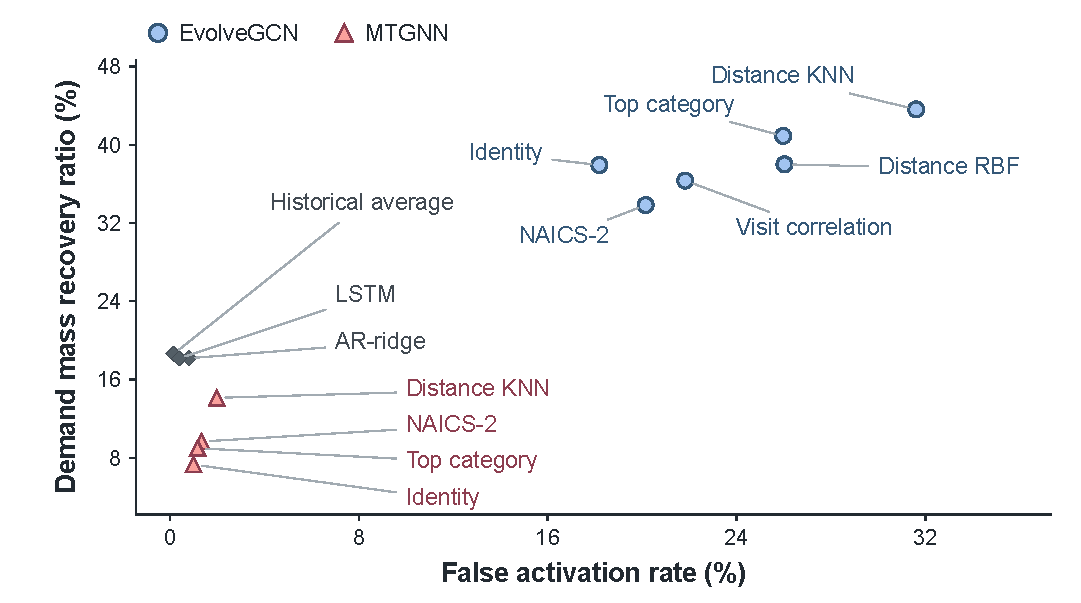
\includegraphics[scale=0.65]{art/recovery_activation_tradeoff.pdf}
\caption{Demand mass recovery ratio (DMR) and false activation rate (FAR) among 1,931 low-history POIs at \(T=14\), \(H=7\). The activation threshold is 0.5 visits. Labels identify adjacency matrices and benchmarks.}
\label{fig:recovery_activation_tradeoff}
\end{figure}

Table~\ref{tab:zero_collapse_diagnostic} reports MAE and RMSE for all test POIs and the remaining diagnostics for the low-history cohort.
Within that cohort, the historical average predicts \(0.19\) visits on average, with a DMR of \(18.6\%\) and a FAR of \(0.16\%\).
LSTM is similarly conservative, with a mean forecast of \(0.18\) visits and a DMR of \(18.2\%\), despite a full-cohort RMSE of \(7.39\).
AR-ridge reduces full-cohort MAE from the historical-average value of \(1.47\) to \(1.43\) and records a DMR of \(18.2\%\) and a FAR of \(0.81\%\) for low-history POIs.
MTGNN reduces aggregate MAE further, with DMR between \(7.3\%\) and \(14.1\%\) across the four reported adjacencies.
The three benchmarks recover a similar fraction of positive demand mass for sparse locations despite differences in full-cohort error.
MTGNN improves overall accuracy while assigning a smaller share of realized demand mass to the positive-visit events of those POIs.

EvolveGCN with identity adjacency recovers \(37.9\%\) of positive demand mass using the visit history of the target POI, with a FAR of \(18.2\%\).
Relative to this within-model reference, top-category adjacency raises DMR to \(40.9\%\) and FAR to \(26.0\%\).
Distance KNN reaches \(43.6\%\) DMR and \(31.6\%\) FAR, the highest values of both metrics among the configurations shown in Figure~\ref{fig:recovery_activation_tradeoff}.
Distance RBF yields a DMR close to the identity result with a higher FAR, while NAICS-2 raises FAR to \(20.2\%\) and reduces DMR to \(33.8\%\).
An upward revision can recover visits on a positive-visit event or produce a false activation on a zero-visit event.
The next analysis examines where these outcomes arise among individual predictions under functional adjacency.

\subsection{Information Sharing among POIs}
\label{subsec:information_sharing_results}


The low-history evaluation shows that information from related POIs affects both positive-demand recovery and false activation.
We further investigate these effects at the individual prediction level and examine how different groups of neighboring POIs contribute to forecast changes.
The analysis combines graph-transfer regime comparisons with neighbor-group perturbations.


\subsubsection{Alternative Adjacency Matrices}
\label{subsubsec:adjacency_results}


We first compare EvolveGCN forecasts under NAICS-2 and identity adjacency to characterize graph-transfer outcomes for individual prediction events.
The former allows information sharing among POIs with the same two-digit NAICS prefix, whereas the latter excludes cross-POI information transfer.
The comparison is conducted at \(T=28\), \(H=14\), covering 407,820 test events from 1,942 low-history POIs.
For each event, graph lift measures the difference between the two forecasts, while target evidence and neighbor evidence summarize historical visits at the target POI and its connected neighbors, respectively.
Combining these measures with observed visits, we identify the graph-transfer regimes reported in Table~\ref{tab:graph_transfer_summary} and evaluate their forecasting performance using MAE gain.


\begin{table}[!t]
\centering
\small
\captionsetup{skip=3pt}
\caption{Graph-transfer regimes under NAICS-2 at \(T=28\), \(H=14\). The shares of positive-demand events and false activations use all events in each regime.}
\label{tab:graph_transfer_summary}
\begingroup
\setlength{\tabcolsep}{3pt}
\renewcommand{\arraystretch}{0.95}
\begin{tabular*}{\linewidth}{@{\extracolsep{\fill}}lrrrrrr@{}}
\toprule
\multicolumn{1}{c}{Regime}
& Events
& Graph lift
& \makecell[c]{Target\\evidence}
& \makecell[c]{Neighbor\\evidence}
& MAE gain
& \makecell[c]{Positive /\\false share} \\
\midrule
Spurious transfer & 10,172 & 0.77 & 0.10 & 6.04 & -0.77 & 0.00 / 1.00 \\
Substitutive transfer & 15,097 & 0.22 & 0.08 & 3.10 & -0.08 & 0.19 / 0.00 \\
Confirmatory transfer & 33,802 & 0.53 & 0.35 & 3.80 & -0.34 & 0.27 / 0.63 \\
Redundant self-history & 150,003 & -0.15 & 0.32 & 1.88 & 0.08 & 0.23 / 0.05 \\
Conservative zero & 151,118 & -0.08 & 0.08 & 1.83 & 0.08 & 0.00 / 0.00 \\
Other & 47,628 & 0.21 & 0.21 & 1.56 & -0.19 & 0.55 / 0.45 \\
\bottomrule
\end{tabular*}
\endgroup
\end{table}

\begin{figure}[!t]
\centering
\captionsetup{skip=3pt}
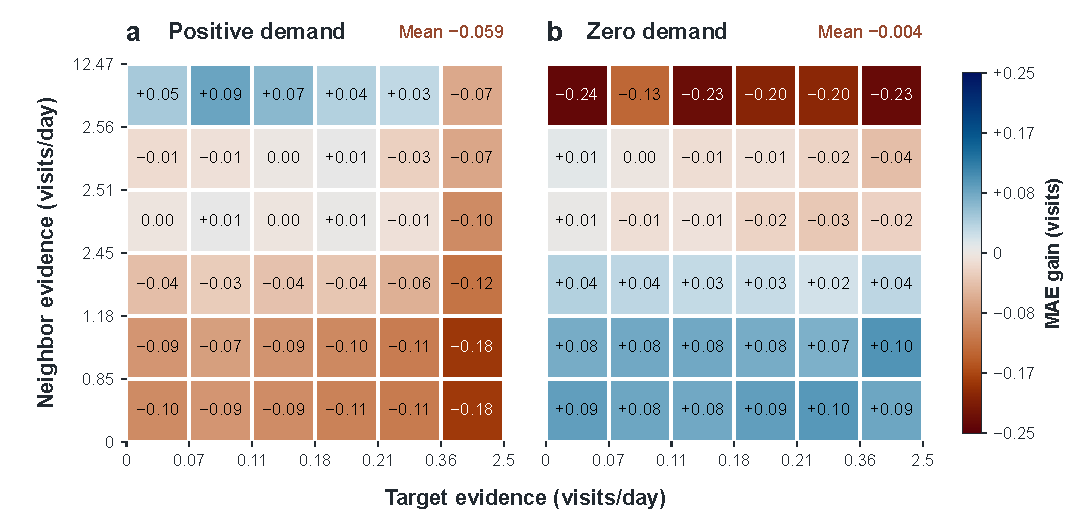
\includegraphics[scale=0.80]{art/outcome_conditioned_graph_transfer.pdf}
\caption{MAE gain of NAICS-2 over identity adjacency at \(T=28\), \(H=14\). Positive gains indicate lower error under NAICS-2. Both panels use pooled evidence sextiles and a common zero-centered color scale. Axis ticks mark bin edges. Panel means weight cells by event count. Cells with fewer than 30 events are marked with a dash.}
\label{fig:counterfactual_graph_transfer_map}
\end{figure}



Table~\ref{tab:graph_transfer_summary} shows that stronger neighbor evidence does not necessarily improve forecasting accuracy for low-history POIs.
Although substitutive and spurious transfer both occur under low target evidence and high neighbor evidence, only \(19.3\%\) of substitutive events have positive observed visits, and their mean MAE gain remains negative at \(-0.08\) visits.
In the spurious regime, a larger mean graph lift of \(0.77\) visits corresponds to an MAE gain of \(-0.77\) visits, indicating that information from active neighbors can substantially overestimate demand at locations with no realized visits.
This limitation also appears in confirmatory transfer, where relatively strong target and neighbor evidence is accompanied by a negative mean MAE gain of \(-0.34\) visits.
In contrast, redundant self-history yields a positive MAE gain of \(0.08\) visits alongside a negative graph lift, suggesting that reducing predicted demand can improve accuracy when the target POI has informative historical observations.
Figure~\ref{fig:counterfactual_graph_transfer_map} further shows that, within the same target and neighbor evidence bins, graph transfer can improve positive-visit forecasts while increasing errors for zero-visit events.
These findings suggest that cross-POI information should be incorporated selectively rather than treating stronger neighbor activity as sufficient evidence of higher demand at the target location.


\begin{table}[!htbp]
\centering
\small
\caption{Substitutive and spurious transfer under functional adjacencies at \(T=28\), \(H=14\).}
\label{tab:semantic_granularity_transfer}
\begin{tabular*}{\linewidth}{@{\extracolsep{\fill}}llrrrr@{}}
\toprule
Adjacency & Regime & Events & Graph lift & MAE gain & Positive / false share \\
\midrule
NAICS-2 & Spurious & 10,172 & 0.77 & -0.77 & 0.00 / 1.00 \\
NAICS-2 & Substitutive & 15,097 & 0.22 & -0.08 & 0.19 / 0.00 \\
NAICS-4 & Spurious & 7,837 & 0.59 & -0.59 & 0.00 / 1.00 \\
NAICS-4 & Substitutive & 9,238 & 0.22 & -0.10 & 0.22 / 0.00 \\
Top category & Spurious & 7,837 & 0.59 & -0.59 & 0.00 / 1.00 \\
Top category & Substitutive & 9,238 & 0.22 & -0.10 & 0.22 / 0.00 \\
\bottomrule
\end{tabular*}
\end{table}


Table~\ref{tab:semantic_granularity_transfer} shows how restricting functional neighbors changes the frequency and accuracy of graph transfer.
Relative to NAICS-2, NAICS-4 reduces the number of substitutive events from 15,097 to 9,238 and raises the positive-visit share among them from \(19.3\%\) to \(21.7\%\).
Mean graph lift remains approximately \(0.22\) visits for both graphs, while mean MAE gain is negative in both substitutive regimes, indicating that more specific functional connections do not necessarily improve prediction accuracy.
NAICS-4 also reduces the number of spurious events from 10,172 to 7,837, with mean MAE gain increasing from \(-0.77\) to \(-0.59\) visits.
The top-category and NAICS-4 adjacencies produce identical results in this comparison.
These findings suggest that restricting functional neighbors changes the frequency and composition of graph transfer more than the magnitude of the remaining substitutive transfers.

\subsubsection{Related-POI Perturbation}
\label{subsubsec:perturbation_results}

We further investigate how different groups of neighboring POIs contribute to graph lift under NAICS-4 adjacency.
For each group, we perturb its historical visit counts while keeping the fitted model and adjacency matrix fixed.
Comparing the full neighborhood with the top-10 active neighbors allows us to assess whether prediction changes are concentrated among highly active POIs, while the correlated and aligned groups examine the contribution of similar temporal visit patterns.
We evaluate these perturbations separately for beneficial and harmful attempted-substitution events.
Beneficial events have positive observed visits and lower absolute error under NAICS-4 than under identity adjacency, whereas harmful events are false activations.
Among beneficial events, recovered positives are those for which the identity forecast is below \(0.5\) visits but the NAICS-4 forecast reaches that threshold.



\begin{table}[!t]
\centering
\fontsize{9pt}{11pt}\selectfont
\captionsetup{skip=3pt}
\caption{Neighbor-group perturbation under NAICS-4 at \(T=28\), \(H=14\). Ben. and harm. refer to beneficial and harmful attempted-substitution events. \(D\) denotes the perturbation effect. A positive \(\Delta\mathrm{MAE}\) indicates higher error after perturbation.}
\label{tab:metric_targeted_perturbation_naics4}
\begingroup
\setlength{\tabcolsep}{2.5pt}
\renewcommand{\arraystretch}{0.95}
\begin{adjustbox}{max width=\linewidth}
\begin{tabular*}{\linewidth}{@{\extracolsep{\fill}}lcccccccc@{}}
\toprule
\makecell[c]{Neighbor\\group}
& \makecell[c]{\(D\)\\Ben.}
& \makecell[c]{\(D\)\\Harm.}
& \makecell[c]{Per node\\Ben.}
& \makecell[c]{Per node\\Harm.}
& \makecell[c]{\(\Delta\mathrm{MAE}\)\\Ben.}
& \makecell[c]{\(\Delta\mathrm{MAE}\)\\Harm.}
& \makecell[c]{False activations\\removed}
& \makecell[c]{Recoveries\\lost} \\
\midrule
All & 0.281 & 0.546 & 0.010 & 0.027 & 0.248 & -0.546 & 0.535 & 0.617 \\
Recent-active & 0.280 & 0.544 & 0.011 & 0.029 & 0.247 & -0.544 & 0.535 & 0.617 \\
High-mean & 0.269 & 0.526 & 0.021 & 0.059 & 0.237 & -0.526 & 0.485 & 0.575 \\
Top-10 active & 0.161 & 0.399 & 0.019 & 0.052 & 0.129 & -0.399 & 0.327 & 0.398 \\
Random-10 & 0.072 & 0.161 & 0.010 & 0.028 & 0.051 & -0.161 & 0.139 & 0.188 \\
Top-10 correlated & 0.060 & 0.134 & 0.009 & 0.025 & 0.039 & -0.134 & 0.128 & 0.164 \\
Aligned & 0.252 & 0.442 & 0.009 & 0.021 & 0.226 & -0.442 & 0.467 & 0.572 \\
Low-mean & 0.035 & 0.037 & 0.001 & 0.004 & 0.030 & -0.037 & 0.052 & 0.086 \\
\bottomrule
\end{tabular*}
\end{adjustbox}
\endgroup
\end{table}

\begin{figure}[!t]
\centering
\captionsetup{skip=3pt}
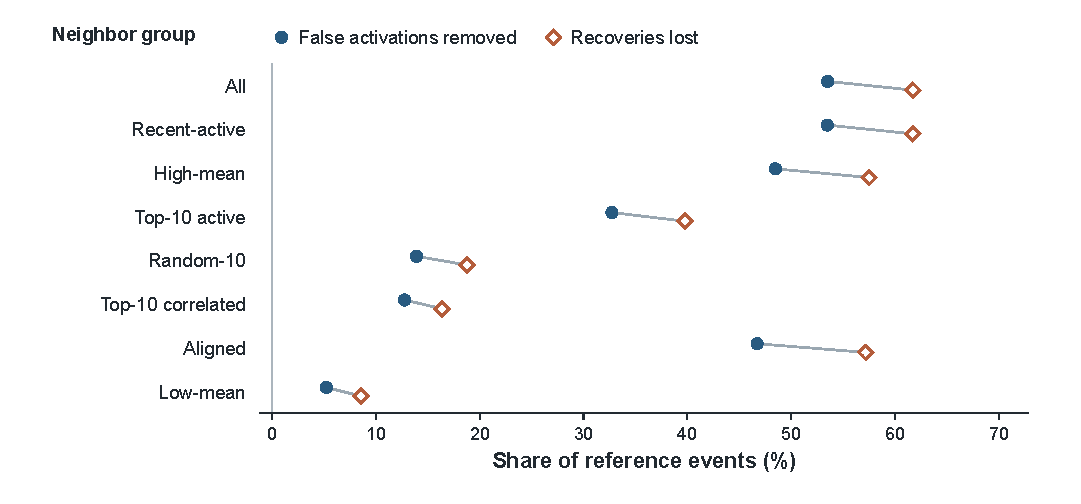
\includegraphics[scale=0.8]{art/neighbor_perturbation_tradeoff.pdf}
\caption{Effect of zeroing neighbor histories under NAICS-4 adjacency at \(T=28\), \(H=14\). Each pair gives the share of false activations removed and the share of positive-demand recoveries lost in their respective reference sets.}
\label{fig:neighbor_perturbation_tradeoff}
\end{figure}


Table~\ref{tab:metric_targeted_perturbation_naics4} shows that perturbing the full neighborhood produces the largest reductions in predicted visits, with nearly identical effects obtained by perturbing recent-active neighbors.
This suggests that recently active POIs account for most of the graph-induced prediction increases.
However, removing this information has opposing effects on beneficial and harmful events.
As shown in Figure~\ref{fig:neighbor_perturbation_tradeoff}, zeroing all neighbor histories eliminates \(53.5\%\) of false activations but also loses \(61.7\%\) of positive-demand recoveries.
The corresponding MAE decreases by \(0.546\) visits for harmful events but increases by \(0.248\) visits for beneficial events.
These results reveal a tradeoff: suppressing neighbor information can correct overprediction at zero-demand locations while removing useful signals for recovering positive demand.

The contribution of neighbor information also varies across groups.
High-mean neighbors have larger effects per perturbed node than the full-neighborhood average, indicating that more active POIs exert greater influence on individual predictions.
However, the top-10 active neighbors account for only \(32.7\%\) of false activations removed and \(39.8\%\) of recoveries lost, suggesting that influential information extends beyond a small number of highly active locations.
Meanwhile, perturbing the top-10 correlated neighbors produces effects comparable to random-10, whereas aligned neighbors account for a substantial share of the prediction changes.
These findings suggest that the intensity and temporal alignment of neighbor activity are more informative about graph lift than correlation-based selection alone.
Nevertheless, the contribution of active neighbors to both beneficial and harmful events indicates that filtering neighbors solely by activity may reduce false activations at the expense of positive-demand recovery.

\subsection{Explaining POI Visit Predictions}
\label{subsec:explanation_results}


Following the analysis of cross-POI information transfer, we further examine how a POI's own historical visits and static attributes contribute to its predictions.
This analysis uses the GNN-static fit with identity adjacency at \(T=14\) and \(H=7\), excluding cross-POI information transfer.
For each POI, the absolute Gradient \(\times\) Input scores are aggregated across test samples and forecast steps and normalized across feature groups to obtain attribution shares.
Examining these shares reveals a strong dominance of location, which has the largest attribution share for 9,806 of the 9,884 POIs (\(99.2\%\)).
Since this dominance obscures differences in reliance on other feature groups, we standardize the attribution shares across POIs and assign each POI to the regime with the highest standardized score.


\subsubsection{POI Attribution Regimes}
\label{subsubsec:attribution_regimes}



Figure~\ref{fig:attribution_fingerprint} reveals substantial heterogeneity in the relative contributions of different information sources across POIs.
Although the parent-driven regime contains only 506 POIs and has a mean original parent share of \(4.0\%\), its standardized parent attribution is \(3.06\) standard deviations above the cohort mean.
This suggests that parent-place information provides a distinctive predictive signal for a relatively small subset of POIs, despite its limited overall contribution.
In contrast, the others-driven regime includes 2,749 POIs, with opening-hour features and their missingness indicators accounting for \(13.1\%\) of the original attribution on average.
These differences suggest that contextual attributes contribute unevenly across locations, motivating a closer examination of how attribution regimes relate to POI functions and forecasting accuracy.


\begin{figure}[htbp]
\centering
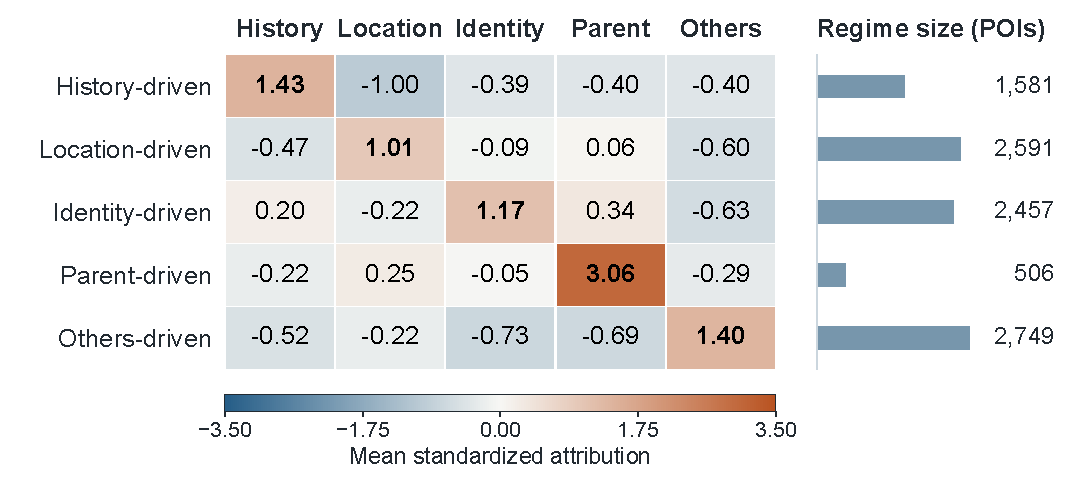
\includegraphics[scale=0.70]{art/attribution_fingerprint.pdf}
\caption{Mean standardized attribution scores and POI counts by regime for the GNN-static fit at \(T=14\), \(H=7\). Positive values indicate shares above the cohort mean for the corresponding source. Bold marks the source that defines each regime.}
\label{fig:attribution_fingerprint}
\end{figure}

\begin{table}[!htbp]
\centering
\fontsize{9pt}{11pt}\selectfont
\captionsetup{skip=5pt}
\caption{Attribution regimes for the GNN-static fit at \(T=14\), \(H=7\). Representative POIs have the smallest Euclidean distances to the mean attribution profile of their regime. Distances use the original attribution shares.}
\label{tab:attri_regime}
\setlength{\tabcolsep}{4pt}
\renewcommand{\arraystretch}{1.15}
\begin{tabularx}{\linewidth}{@{}lr>{\raggedright\arraybackslash}Xr@{}}
\toprule
Regime & POIs & Representative POIs & MAE \\
\midrule
History-driven & 1,581 & The Polyclinic Plastic Surgery at Nordstrom Tower, Trask Orthodontics, Eighteen15 Bar & 3.108 \\
Location-driven & 2,591 & Southsea Spices, Lennar at High Point, The Laser Dome & 1.629 \\
Identity-driven & 2,457 & Freed Art Design, J \& J Auto Master, ANT Autoworks & 1.153 \\
Parent-driven & 506 & Tecnicolfs llc, 2bar Spirits, The Landing at Tyee on Lake Union & 1.415 \\
Others-driven & 2,749 & CDI (Center for Diagnostic Imaging), Cafe 5ive, Theo Chocolate & 1.298 \\
\bottomrule
\end{tabularx}
\end{table}


Table~\ref{tab:attri_regime} shows differences in forecasting accuracy across attribution regimes.
The history-driven regime has the highest MAE of \(3.108\) visits, compared with \(1.153\) visits for the identity-driven regime, indicating that prediction difficulty varies with the information sources on which models rely.
These attribution patterns also differ across urban functions, as shown in Table~\ref{tab:category_regime_mae}.
Among schools, campuses, and education-related POIs, \(81.3\%\) are identity-driven, whereas \(55.6\%\) of grocery and daily retail POIs are location-driven.
The others-driven regime is more prevalent among bars and nightlife (\(44.4\%\)) and restaurants and cafes (\(38.7\%\)), reflecting greater relative reliance on opening-hour information and its missingness indicators.
These differences suggest that the information underlying POI forecasts varies systematically across urban functions, rather than following a uniform prediction mechanism.


\begin{table}[!htb]
\centering
\fontsize{9pt}{11pt}\selectfont
\caption{Attribution-regime shares within broad POI categories. H, L, I, P, and O denote history-driven, location-driven, identity-driven, parent-driven, and others-driven, respectively. MAE uses the same GNN-static predictions.}
\label{tab:category_regime_mae}
\setlength{\tabcolsep}{3.5pt}
\renewcommand{\arraystretch}{1.12}
\begin{tabularx}{\linewidth}{@{}>{\raggedright\arraybackslash}Xrrrrrrr@{}}
\toprule
POI category & POIs & H (\%) & L (\%) & I (\%) & P (\%) & O (\%) & MAE \\
\midrule
Bars and nightlife POIs & 383 & 16.2 & 16.2 & 20.9 & 2.3 & 44.4 & 1.308 \\
Clinics and medical services & 1,090 & 15.0 & 27.6 & 32.6 & 9.4 & 15.3 & 1.656 \\
Grocery and daily retail & 423 & 15.6 & 55.6 & 0.2 & 8.5 & 20.1 & 1.825 \\
Pharmacies and health-related retail & 240 & 22.5 & 48.3 & 1.7 & 3.8 & 23.8 & 1.789 \\
Repair, towing, and irregular services & 283 & 13.4 & 9.9 & 30.4 & 2.1 & 44.2 & 1.106 \\
Restaurants and cafes & 2,604 & 13.1 & 18.7 & 24.9 & 4.6 & 38.7 & 1.720 \\
Schools, campuses, and education-related POIs & 294 & 5.4 & 2.7 & 81.3 & 2.4 & 8.2 & 1.577 \\
Shopping centers and office-building POIs & 2,879 & 16.4 & 34.6 & 28.9 & 4.2 & 15.9 & 1.648 \\
Small local businesses & 1,688 & 21.8 & 21.1 & 12.4 & 5.7 & 38.9 & 1.627 \\
\bottomrule
\end{tabularx}
\end{table}

\begin{figure}[!htb]
\centering
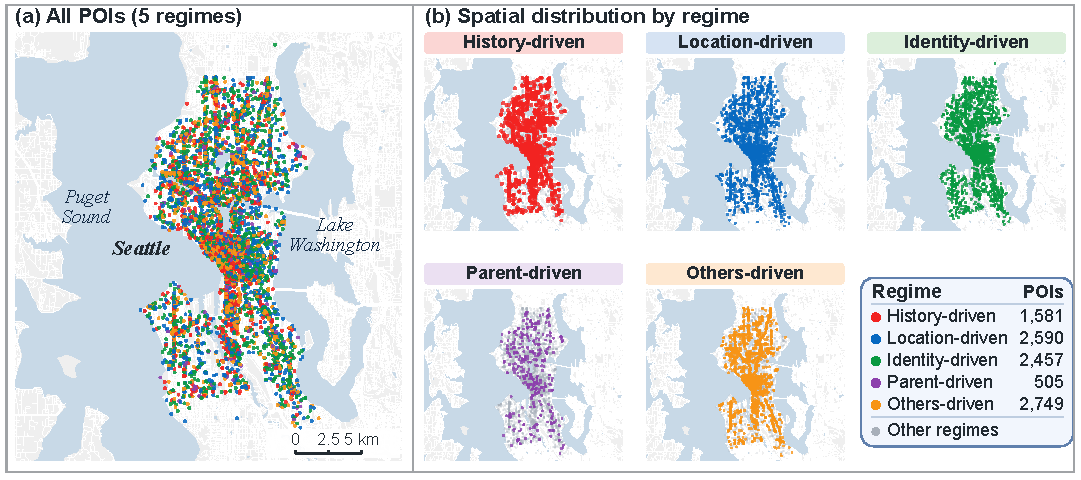
\includegraphics[width=\linewidth]{art/attribution_cluster_map.pdf}
\caption{Spatial distribution of the five attribution regimes in Seattle. The overview shows the regimes together. Each small panel highlights one regime and shows the other POIs in gray. Legend counts refer to the 9,882 POIs within the mapped extent. Road and water features are from the 2020 U.S. Census Bureau TIGER/Line files.}
\label{fig:attribution_regime_map}
\end{figure}


Figure~\ref{fig:attribution_regime_map} illustrates the spatial distribution of the five attribution regimes across Seattle.
The regimes exhibit substantial geographic overlap rather than forming distinct spatial regions, with POIs assigned to different regimes frequently appearing near one another.
This pattern suggests that geographic proximity alone does not determine which information sources contribute most strongly to POI predictions, highlighting the heterogeneity of prediction mechanisms even within the same urban area.

\subsubsection{Parent-Place Information}
\label{subsubsec:parent_results}

POIs located within larger destinations, such as shopping malls and medical facilities, may share contextual characteristics with their parent places.
We further examine how parent-place information contributes to forecasts for these embedded POIs relative to their own historical visits and other static attributes.
The analysis covers 581 POIs with recorded parent places and compares attribution patterns across different embedded POI groups.


\begin{table}[!htbp]
\centering
\fontsize{9pt}{11pt}\selectfont
\caption{Mean attribution shares for POIs with a recorded parent place. Selected subgroups use the top category of the embedded POI. Gap is the parent share minus the combined share of the other sources, computed before rounding.}
\label{tab_parent}
\begingroup
\setlength{\tabcolsep}{4pt}
\renewcommand{\arraystretch}{1.12}
\begin{tabular*}{\linewidth}{@{\extracolsep{\fill}}lccccc@{}}
\toprule
Embedded POI group
& POIs
& Parent (\%)
& Other (\%)
& Gap (pp)
& MAE \\
\midrule
Cafes and restaurants
& 181 & 3.4 & 96.6 & -93.2 & 1.874 \\
Pharmacies and health retail
& 18 & 3.3 & 96.7 & -93.4 & 2.240 \\
Retail and service shops
& 126 & 3.3 & 96.7 & -93.4 & 1.743 \\
Education-related POIs
& 8 & 4.5 & 95.5 & -91.0 & 2.182 \\
Medical and clinic-related POIs
& 61 & 3.9 & 96.1 & -92.2 & 3.557 \\
\midrule
All embedded POIs
& 581 & 3.8 & 96.2 & -92.5 & 1.870 \\
\bottomrule
\end{tabular*}
\endgroup
\end{table}

Table~\ref{tab_parent} shows that parent-place information accounts for only \(3.8\%\) of mean attribution across embedded POIs, while the remaining information sources contribute \(96.2\%\).
The parent attribution share remains between \(3.3\%\) and \(4.5\%\) across the displayed groups, indicating that the model relies primarily on POI-specific information even when establishments are located within larger destinations.
This pattern suggests that parent-place context serves as a supplementary signal, while individual visit histories and other attributes remain central to interpreting establishment-level demand forecasts.
The medical and clinic-related group has the highest MAE of \(3.557\) visits among the reported groups, highlighting the value of assessing forecasting accuracy separately for these establishments when supporting local service planning.


\subsubsection{Category and Industry Granularity}
\label{subsubsec:granularity_results}

Finally, we examine how category labels and industry codes at different levels of granularity contribute to POI visit predictions, identifying which semantic descriptors have the largest attribution.
Specifically, top category, sub-category, NAICS-2, and NAICS-4 are encoded jointly in the GNN-static fit, with each descriptor's attribution share computed relative to all feature groups.
For events with nonzero semantic attribution, the descriptor with the largest attribution among the four determines the dominant-event subset used to calculate conditional MAE.
This allows us to compare the relative contributions of semantic representations and the forecasting accuracy associated with their dominance.

\begin{table}[!htbp]
\centering
\fontsize{9pt}{11pt}\selectfont
\caption{Attribution of four semantic descriptors in the GNN-static fit. Mean share uses total attribution across all sources. Dominance is assessed among the four descriptors for events with nonzero semantic attribution.}
\label{tab:semantic_granularity}
\begingroup
\setlength{\tabcolsep}{4pt}
\renewcommand{\arraystretch}{1.12}
\begin{tabular*}{\linewidth}{@{\extracolsep{\fill}}lcccc@{}}
\toprule
\makecell[l]{Descriptor}
& \makecell[c]{Mean share\\(\%)}
& \makecell[c]{Dominance\\(\%)}
& \makecell[c]{Dominant-event\\MAE}
& \makecell[c]{Dominant\\events} \\
\midrule
Top category & 2.00 & 11.35 & 1.760 & 172,798 \\
Sub-category & 1.74 & 3.92 & 2.138 & 59,644 \\
NAICS-2 & 3.07 & 66.81 & 1.536 & 1,016,983 \\
NAICS-4 & 2.17 & 17.92 & 1.866 & 272,711 \\
\bottomrule
\end{tabular*}
\endgroup
\end{table}


Table~\ref{tab:semantic_granularity} shows that NAICS-2 is the dominant semantic descriptor in \(66.81\%\) of eligible events and has the largest mean attribution share (\(3.07\%\)).
This concentration indicates that broad industry classifications provide the most prominent semantic signal for most eligible predictions, despite the simultaneous inclusion of more detailed descriptors.
NAICS-2-dominant events also have the lowest conditional MAE (\(1.536\) visits), although this comparison reflects differences across event subsets rather than the independent effect of each descriptor.
In contrast, the graph-transfer analysis at \(T=28\) and \(H=14\) shows fewer spurious transfer events under NAICS-4 adjacency than under NAICS-2, as reported in Table~\ref{tab:semantic_granularity_transfer}.
These findings reveal different roles for semantic granularity in POI representation and neighbor selection, with broad industry classifications dominating semantic attribution and more specific functional connections associated with fewer spurious transfers.


\section{Conclusions and future work}
\label{conclude}

This paper studies POI visit forecasting under sparse and heterogeneous urban demand, motivated by the need to understand not only future location-level activity but also the information sources behind model predictions. Unlike conventional forecasting studies that mainly compare aggregate accuracy, this study treats POI forecasting as both a predictive and an interpretive problem. 
This perspective is important because sparse POIs may be systematically underestimated by conservative baselines, while graph-based models may improve demand recovery only when contextual information is transferred in a reliable manner.

To address this problem, we developed an explainable temporal graph learning framework that integrates visit histories, POI relationships, and static contextual attributes. The framework evaluates two representative temporal graph models, MTGNN and EvolveGCN, against non-graph baselines under multi-horizon forecasting settings. In addition to standard forecasting metrics, we introduced zero-demand-collapse diagnostics to examine whether models can recover realized positive demand for low-history POIs without generating excessive false activations. We further used perturbation-based graph-transfer analysis and attribution-regime analysis to examine how spatial, semantic, temporal, and operational signals contribute to location-level forecasts.

The empirical results show that graph neural forecasting provides a nuanced rather than uniform advantage. Historical averages remain a strong benchmark for aggregate forecasting, particularly at longer horizons where the task is closely related to estimating each POI's typical demand level. 
MTGNN achieves the lowest aggregate MAE across all four input-window and forecast-horizon settings, while EvolveGCN with identity adjacency recovers more positive demand mass among low-history POIs at the cost of additional false activations.
Perturbing all neighbor histories eliminates \(53.5\%\) of false activations but also loses \(61.7\%\) of positive-demand recoveries, with recently active neighbors accounting for nearly all of these changes.


The attribution analysis further shows that POI forecasts are generated through heterogeneous mechanisms. 
Some locations exhibit stronger relative reliance on historical visits, whereas others show greater relative contributions from location, functional identity, parent-place context, or other static attributes.
The regime-level results reveal how the same forecasting architecture relies on different information sources across urban functions.
They also show that more detailed semantic information does not necessarily lead to better predictions, as broad industry classifications dominate semantic attribution while finer functional connections are associated with fewer spurious transfers.
These findings suggest that explainable POI forecasting should evaluate not only prediction error, but also the reliability and source of contextual information used by the model.

Several future research directions remain. First, future work could test the proposed framework using longer observation periods, multiple cities, and additional mobility datasets to examine whether the identified forecasting and attribution regimes are stable across urban contexts. Second, richer exogenous variables, such as weather, special events, accessibility, and neighborhood conditions, could be incorporated to separate regular visitation patterns from external demand shocks. Third, selective or uncertainty-aware graph propagation methods could be developed to control the recovery--false-activation tradeoff for sparse POIs. Finally, future work may connect explainable POI forecasts with downstream planning models, so that the value of interpretability can be assessed through its contribution to service design, facility location, transit planning, and other operational decisions.

\newpage
\begingroup
\singlespacing
\bibliographystyle{abbrvnat}
\bibliography{reference}
\endgroup

\end{document}
